\chapter{Search for standard model~\tttt production in \runtwo at $\sqrt{s} =$~13~TeV \label{c:Run2}}
\section{Introduction}
In this chapter, an analysis of the full 2015 CMS data set of proton-proton collisions at $\sqrt{s} =$~13~TeV with 2.6~\fbinv of data is presented where the SM production of four top quarks (\tttt) is sought. SM \tttt production has a cross section of $\sigmattttSM \approx 9.2$ fb at NLO with NNLO corrections~\cite{Alwall2014,Bevilacqua2012}. 

All sections apart from the training of the hadronic top quark reconstruction in Section~\ref{sec:topContent13} are the authors personal contribution to the analysis.

\section{Data and Simulation}
\label{sec:datasimulation13}
This analysis uses data from proton-proton collision at the CMS experiment in 2015 at $\sqrt{s}=13$~TeV.
Data were collected using a trigger based on the presence of at least one muon (electron) candidate with $\pt > $~18~(23)~GeV for the muon (electron) channel and corresponds to an integrated luminosity of 2.6~\fbinv .
% The full 2012 SingleElectron dataset is used for the electron channel, which requires an electron candidate with $\pt > $ 27 GeV and corresponds to an integrated luminosity of 19.7 \fbinv.
The signal SM \tttt MC samples and the background MC samples are given in table~\ref{tab:datasets_sim_13tev}, along with the MC generator used to produce these samples, the order at which they were produced and the number of events produced. MC samples were produced for the hadronisation scale systematic, which can be found in table~\ref{tab:datasets_sys_13tev}. In this analysis the ME scale and PS scale are treated as separate uncertainties.

\begin{table}[ht!]
% \tiny
\centering
\begin{tabular}{| l | l | l | p{2cm} |}
 \hline 
 Dataset & Events & Generator & Order \\
\hline
\tttt & 960K & \MADGRAPH\aMCATNLO & NLO \\
\hline
\ttbar &97M & \POWHEG  & NLO \\
\hline
WJetsToLNu & 47M & \MLM & NLO \\
\hline
Tbar\_tW-channel & 1M & \POWHEG & NLO\\
\hline
T\_tW-channel & 1M & \POWHEG & NLO \\
\hline
DYJetsToLL & 9M & \MLM & NLO \\
\hline
TTZJets  & 400K & \MADGRAPH\aMCATNLO & NLO \\
\hline
TTWJets\ & 250K & \MADGRAPH\aMCATNLO & NLO \\
\hline
TTH\_HToBB & 4M & \POWHEG & NLO \\
% \hline
% ZZ & 10M & \PYTHIA 6 & O \\
% \hline
% WZ &10M & \PYTHIA 6 & O \\
% \hline
% WW &10M & \PYTHIA 6 & O \\
\hline
\end{tabular}
 \caption{Dataset name, total number of events, MC generator and order of the simulated samples. \PYTHIA~8 is used to hadronise all samples in this table.}
  \label{tab:datasets_sim_13tev}
  \end{table}


\begin{table}[ht!]
% \tiny
\centering
\begin{tabular}{| l | l | l | p{2cm} |}
 \hline 
 Dataset & Events & Generator & Order \\
\hline
TTJets\_scaledown & 10M  & \POWHEG & NLO \\
\hline
TTJets\_scaleup & 10M  & \POWHEG & NLO \\
\hline
TTJets & 5M & \MLM & NLO  \\
\hline
TTJets & 5M & \MADGRAPH\aMCATNLO~FxFx & NLO \\
\hline
\end{tabular}
 \caption{Dataset name, total number of events, MC generator and order of the simulated systematic samples. \PYTHIA~8 is used to hadronise all samples in this table.}
  \label{tab:datasets_sys_13tev}
\end{table}

\section{Baseline Event Selection}
\label{sec:baseline13}
The set of criteria applied to the reconstructed objects in events, which are triggered by the single muon or single electron triggers, to preferentially select \tttt events and suppress background events is detailed below.

For the muon channel these are:
\begin{itemize}
\setlength\itemsep{0em}
\item Exactly one tight muon
\item Exactly zero additional loose muons
\item Exactly zero loose electrons
\item At least 6 jets with $\pt >$ 30 \GeV
\item At least 2 CSVM tagged b-jets
\end{itemize}
For the electron channel these are:
\begin{itemize}
\itemsep0em 
\item Exactly one tight electron
\item Exactly zero additional loose electrons
\item Exactly zero loose muons
\item At least 6 jets with $\pt >$ 30 \GeV
\item At least 2 CSVM tagged b-jets
\end{itemize}

\section{Corrections to the simulation}
\label{sec:Calibrations13}
All corrections are described in Section~\ref{sec:Calibrations}. The PU corrections are applied, producing a good agreement in the distribution of the number of vertices as seen in Fig.~\ref{fig:PUReWeight13}. Muon scale factors~\cite{muonSFtwiki} and electron scale factors~\cite{electronSFtwiki} are applied. By comparing the efficiencies in data with the efficiencies in simulation, a value was obtained of $1.0001\pm0.0001$ for the electron trigger scale factor which was taken to be 1 in the analysis. 

\begin{figure}[h!]
\begin{center}
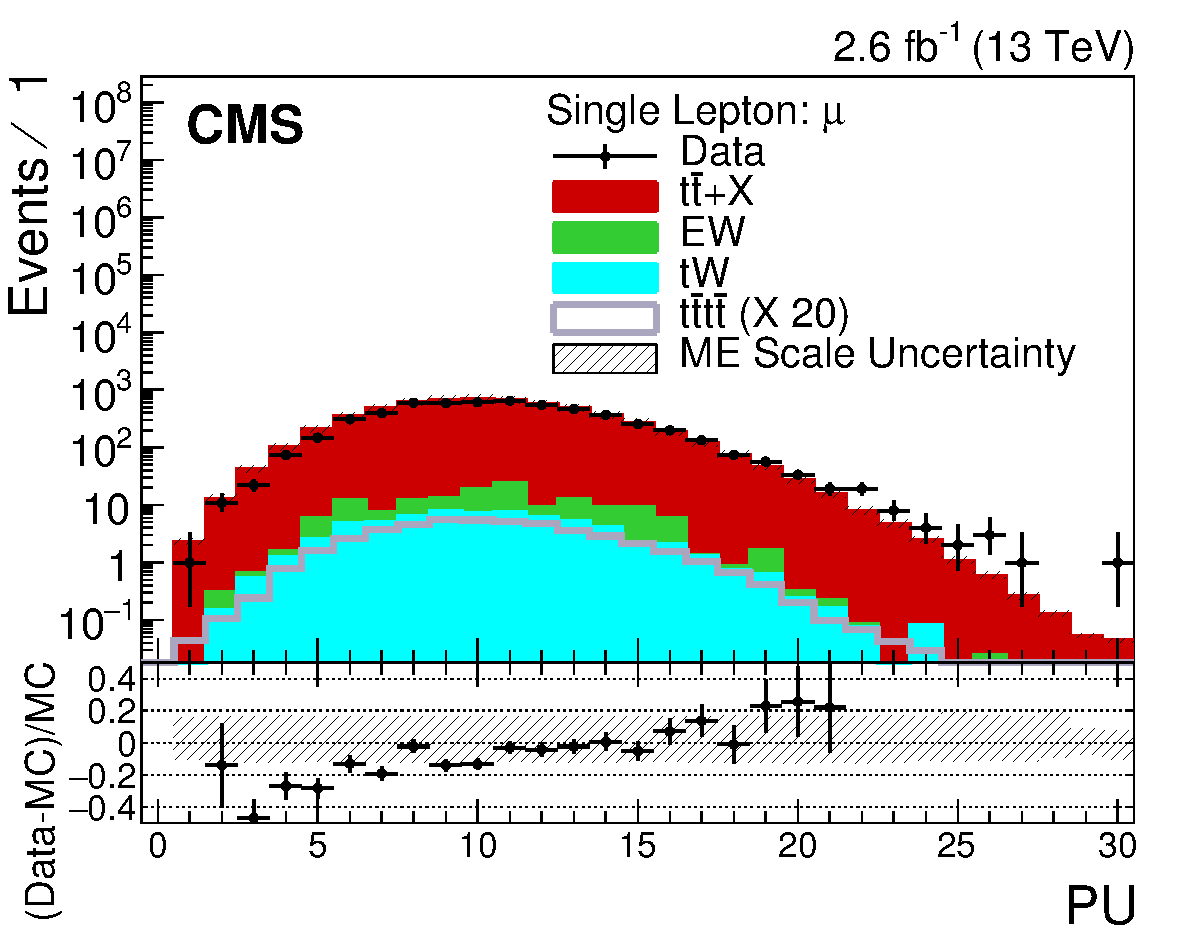
\includegraphics[width=0.67\textwidth]{images/Run2/PU_StackLogY.pdf}
\end{center}
\caption{The number of primary vertices for data and simulation after application of PU corrections for $\mu$ + jets.}
\label{fig:PUReWeight13}
\end{figure}

The method in Section~\ref{subsec:method2btag} was used to derive the b tagging scale factors. Figures~\ref{fig:csvJet3SF} and~\ref{fig:csvJet4SF} show the effect of applying the b-tagging scale factor to correct the CSV discriminator distributions and it can be seen that the agreement between data and simulation has been improved.

\begin{figure}[ht!]
    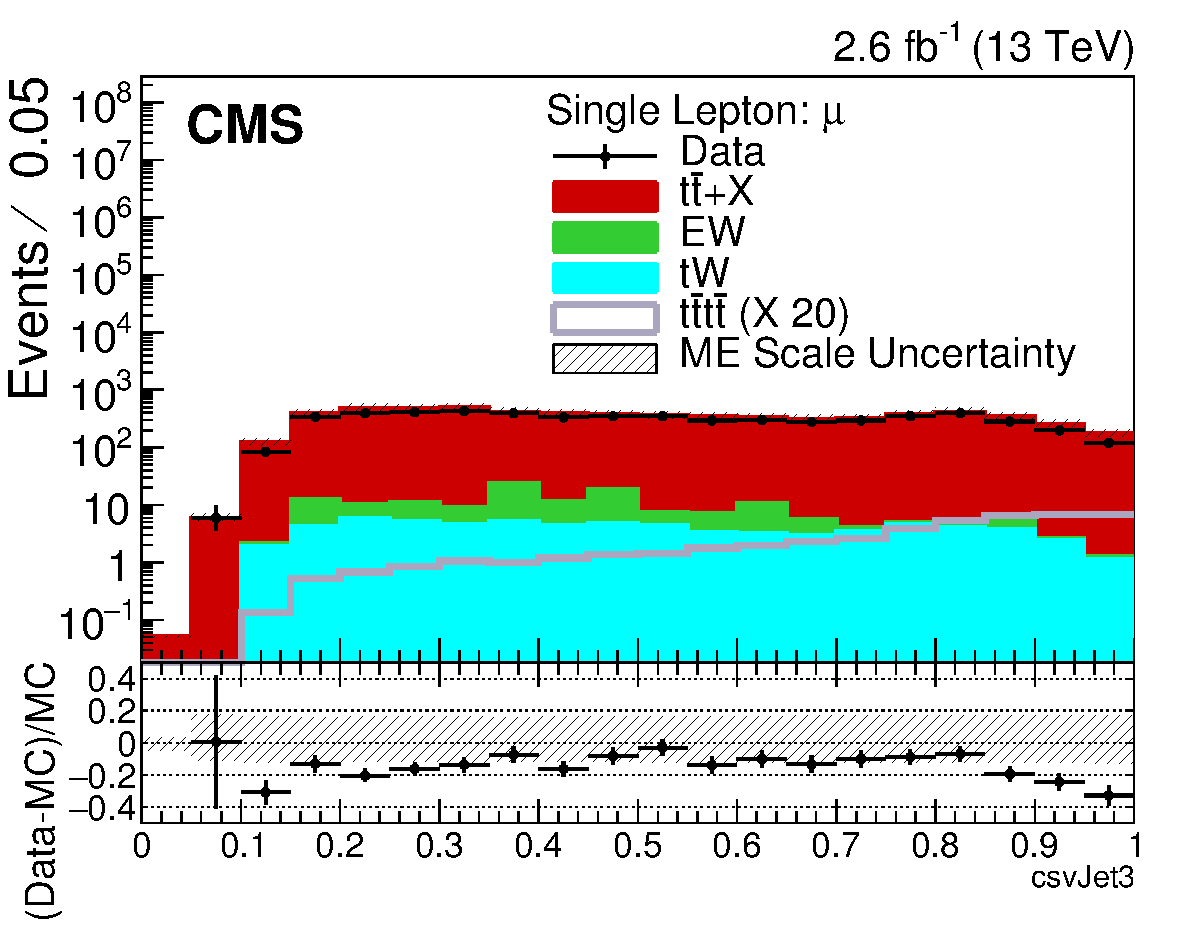
\includegraphics[width=0.48\textwidth]{images/Run2/csvJet3_StackLogY_noSF.pdf}
    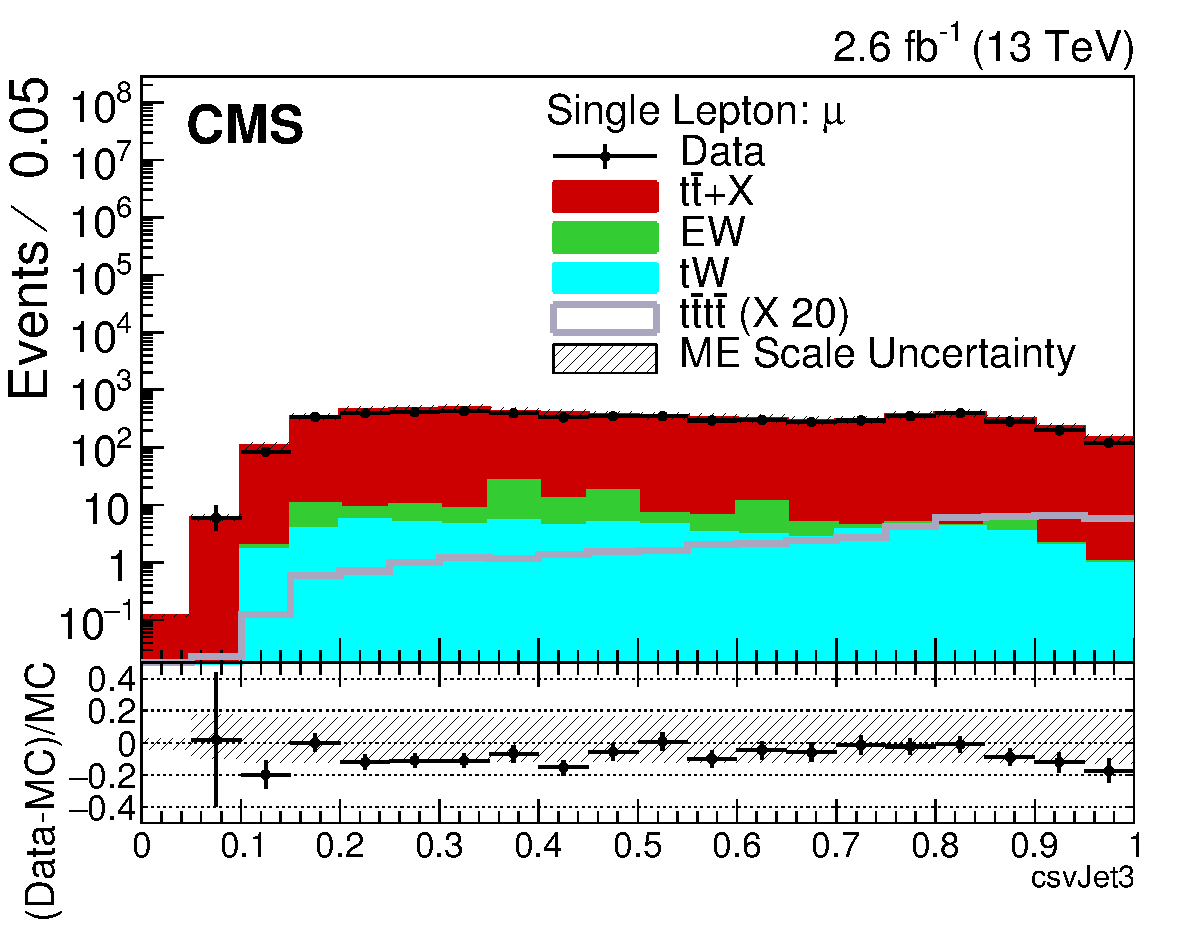
\includegraphics[width=0.48\textwidth]{images/Run2/csvJet3_StackLogY.pdf}
    \caption{ The third-highest ranked CSV jet distributions for data and simulation event in the $\mu$ + jets channel (left) and $e$ + jets channel (right) are plotted.}
    \label{fig:csvJet3SF}
\end{figure}
\begin{figure}[ht!]
    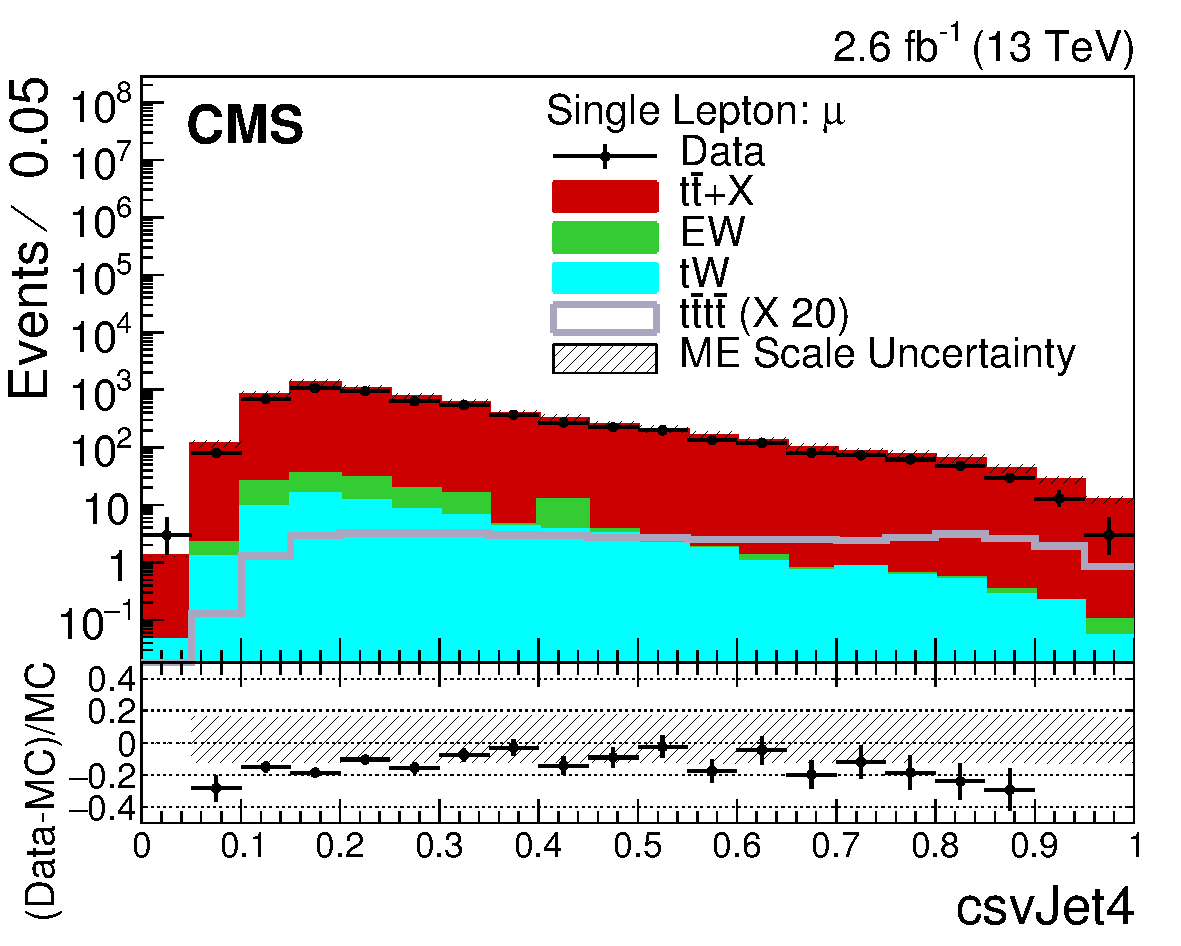
\includegraphics[width=0.48\textwidth]{images/Run2/csvJet4_StackLogY_noSF.pdf}
    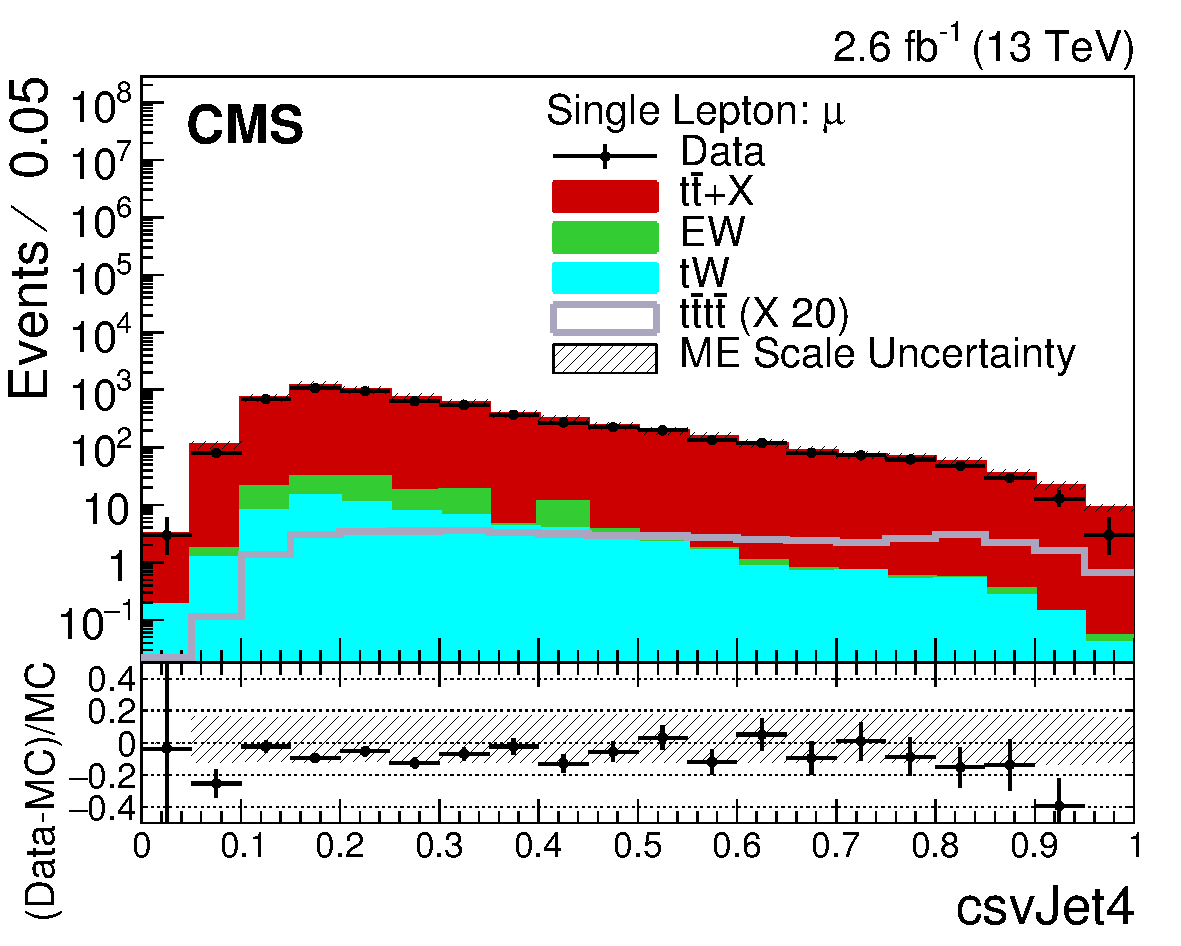
\includegraphics[width=0.48\textwidth]{images/Run2/csvJet4_StackLogY.pdf}
    \caption{ The fourth-highest ranked CSV jet distributions for data and simulation event in the $\mu$ + jets channel (left) and $e$ + jets channel (right) are plotted.}
    \label{fig:csvJet4SF}
\end{figure}
 

The jet multiplicity modelling from Section~\ref{subsec:alphaS} was applied. It can be seen from Figs.~\ref{fig:withAlpha} and~\ref{fig:withoutAlpha} that the jet multiplicity modelling is greatly improved by applying this correction.

\begin{figure}[ht!]
    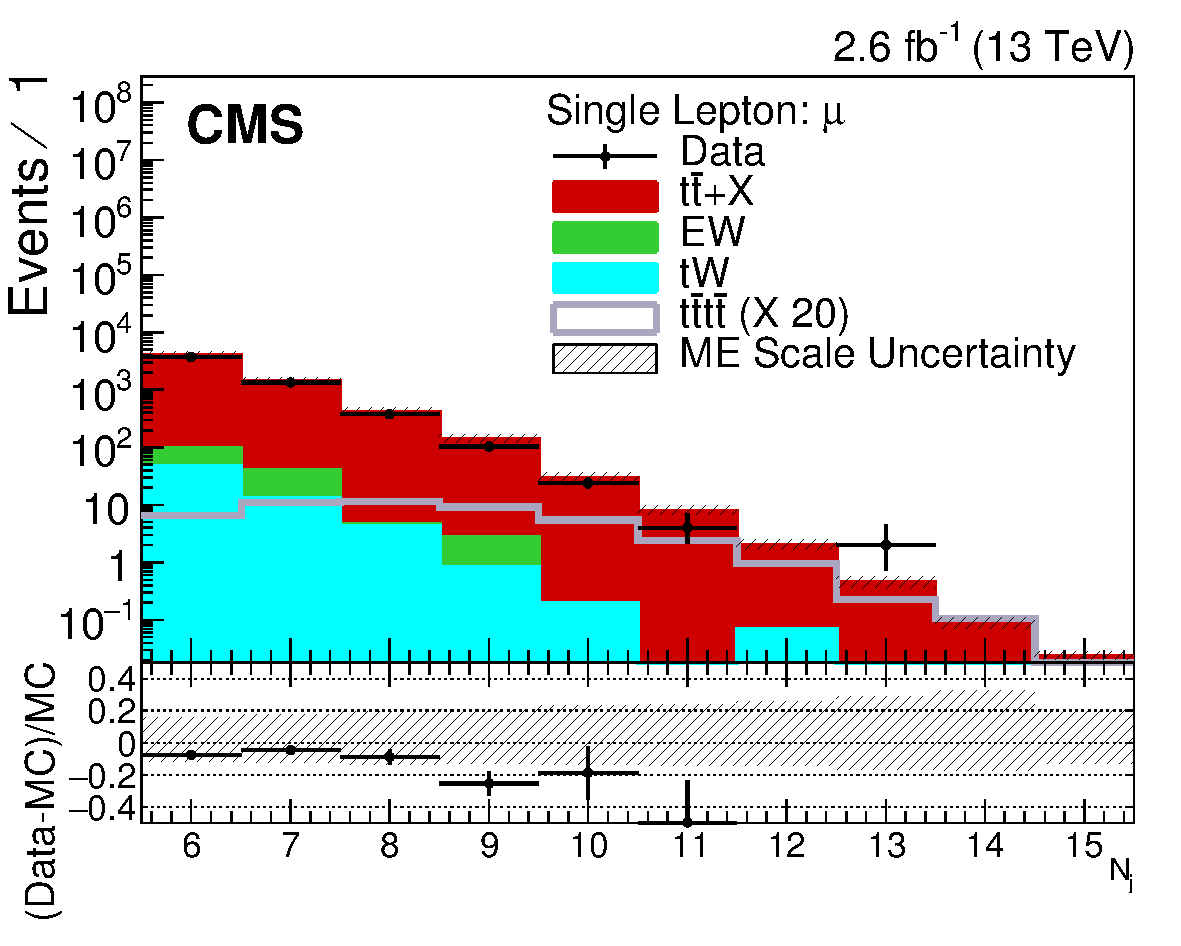
\includegraphics[width=0.48\textwidth]{images/Run2/nJets_StackLogY.pdf}
    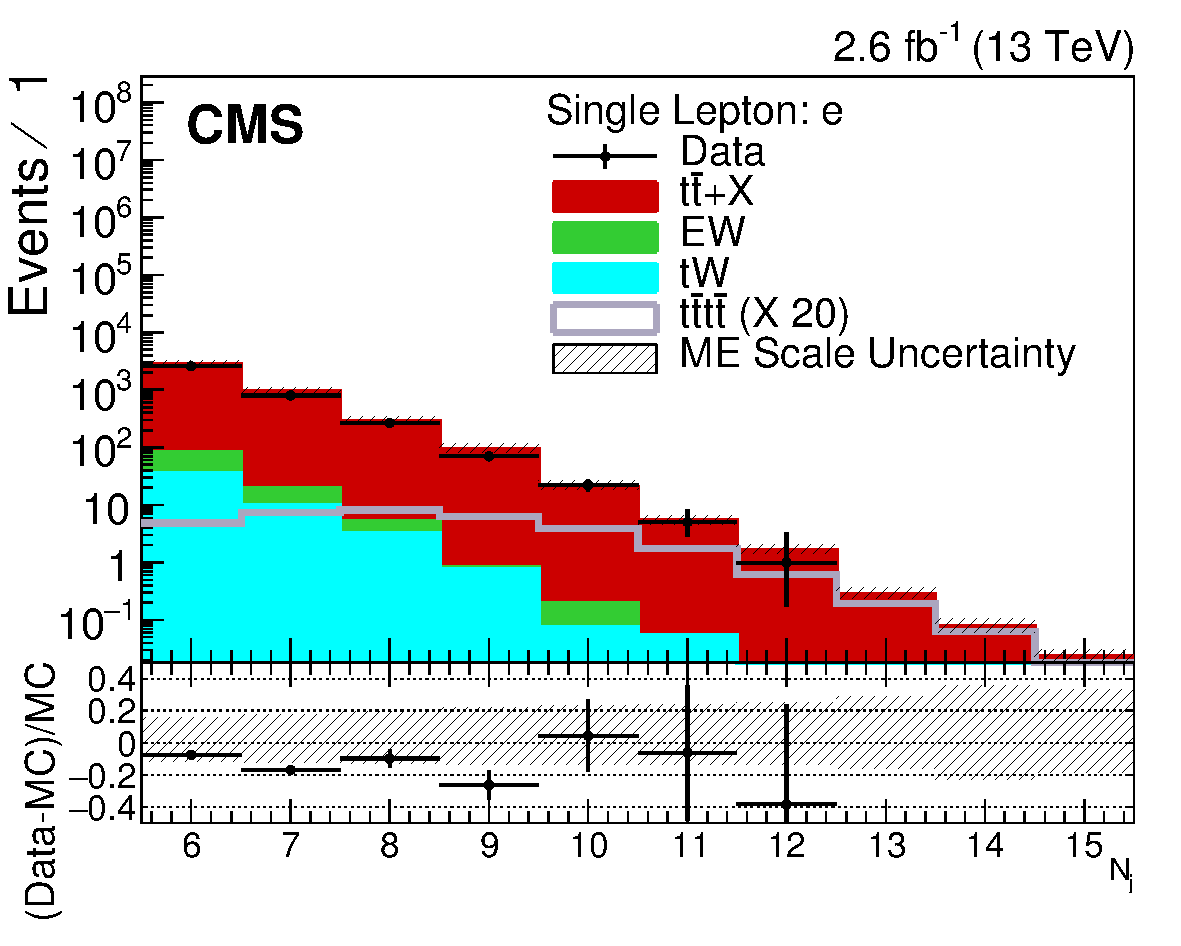
\includegraphics[width=0.48\textwidth]{images/Run2/nJets_StackLogY_e.pdf}
    \caption{The \njets distributions for data and simulation in the $\mu$ + jets channel (left) and $e$ + jets channel (left) with jet multiplicity modelling scale factors applied.}
    \label{fig:withAlpha}
\end{figure}

\begin{figure}[ht!]
    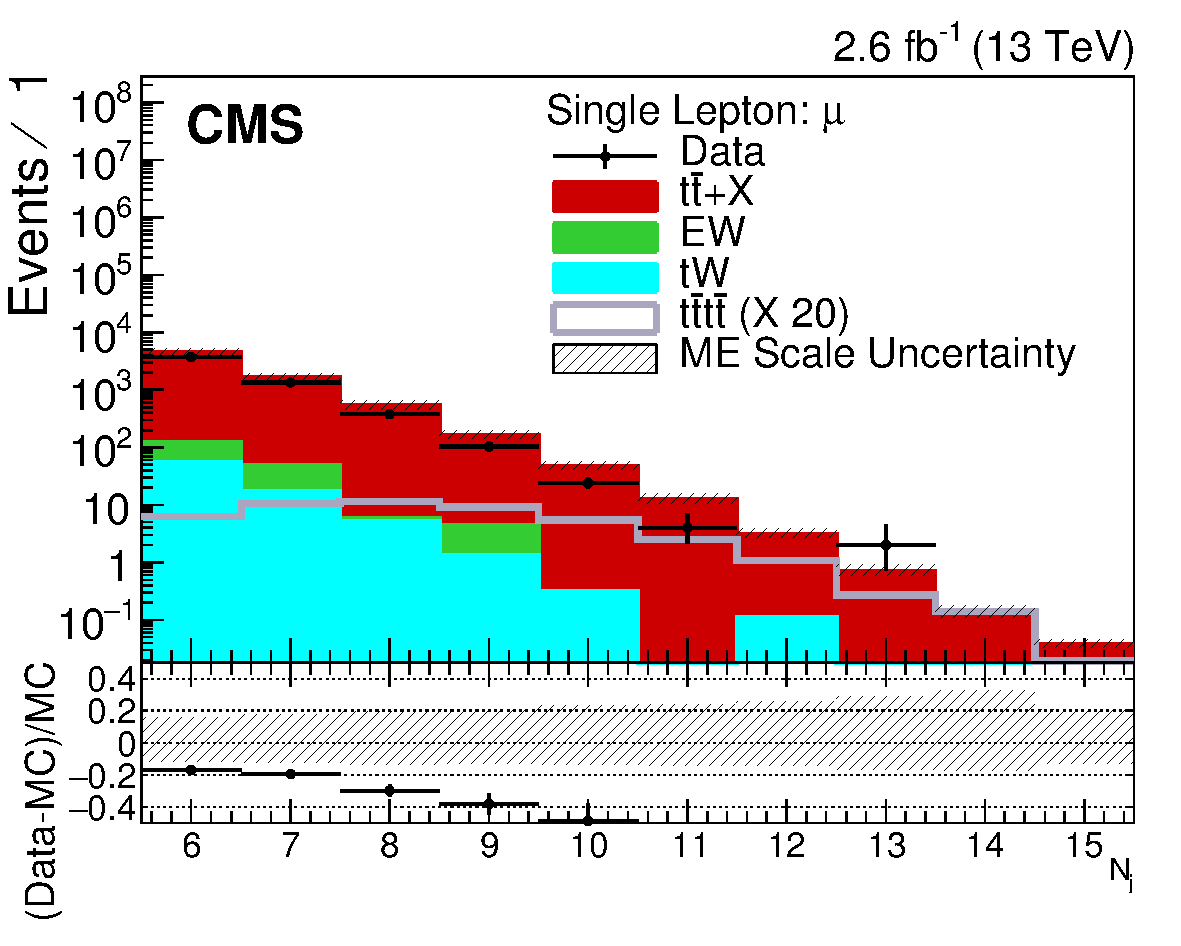
\includegraphics[width=0.48\textwidth]{images/Run2/nJets_StackLogY_woAlphaS.pdf}
    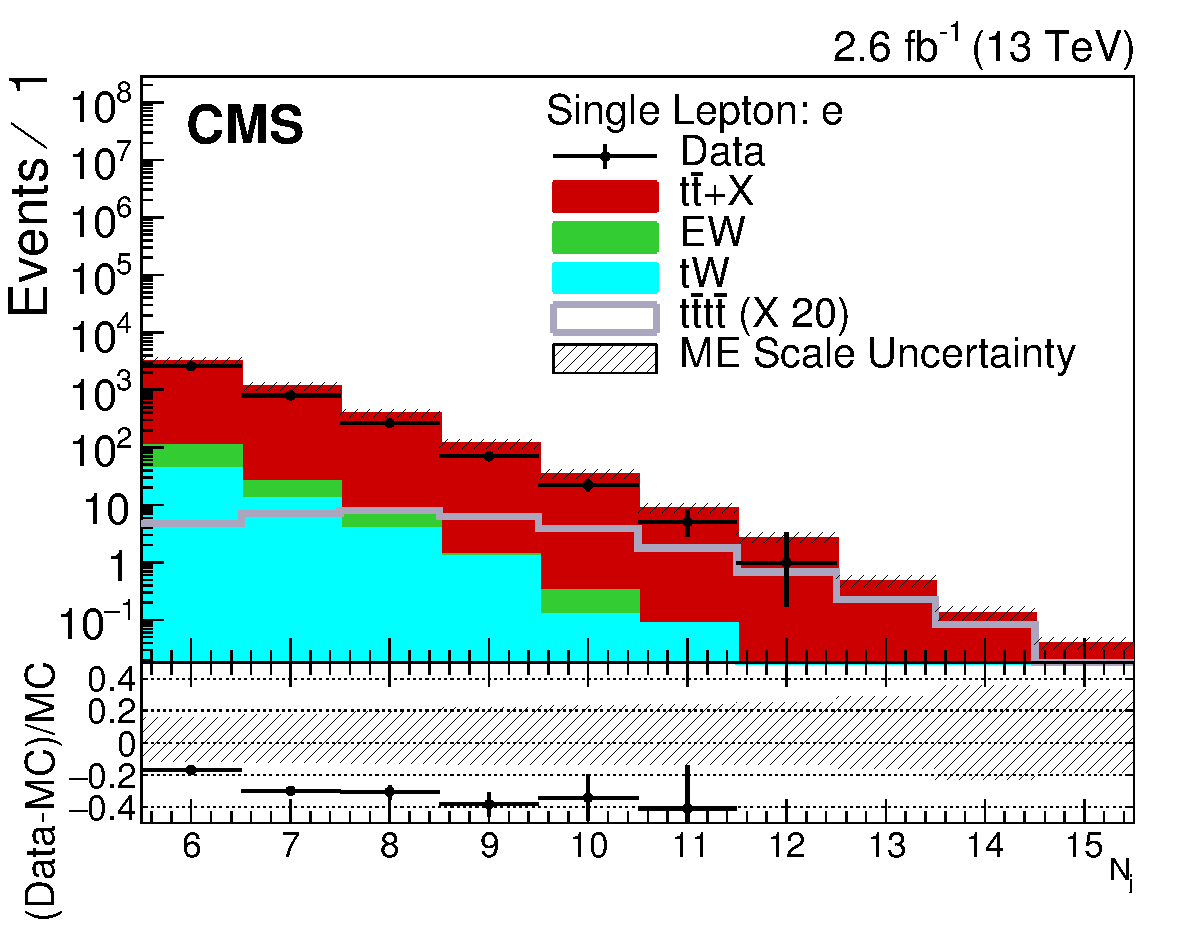
\includegraphics[width=0.48\textwidth]{images/Run2/nJets_StackLogY_e_woAlphaS.pdf}
    \caption{The \njets distributions for data and simulation in the $\mu$ + jets channel (left) and $e$ + jets channel (left) without jet multiplicity modelling scale factors applied.}
    \label{fig:withoutAlpha}
\end{figure}

The scale factors applied for the heavy flavour modelling are described in Section~\ref{ttbbmod}. The distributions for the \nMtags are shown with and without the heavy flavour modelling scale factors applied. It is not obvious that there is a significant improvement in the \nMtags after the scale factors have been applied but the heavy flavour fraction is allowed to float as a shape nuisance parameter in the template fit.

\begin{figure}[ht!]
    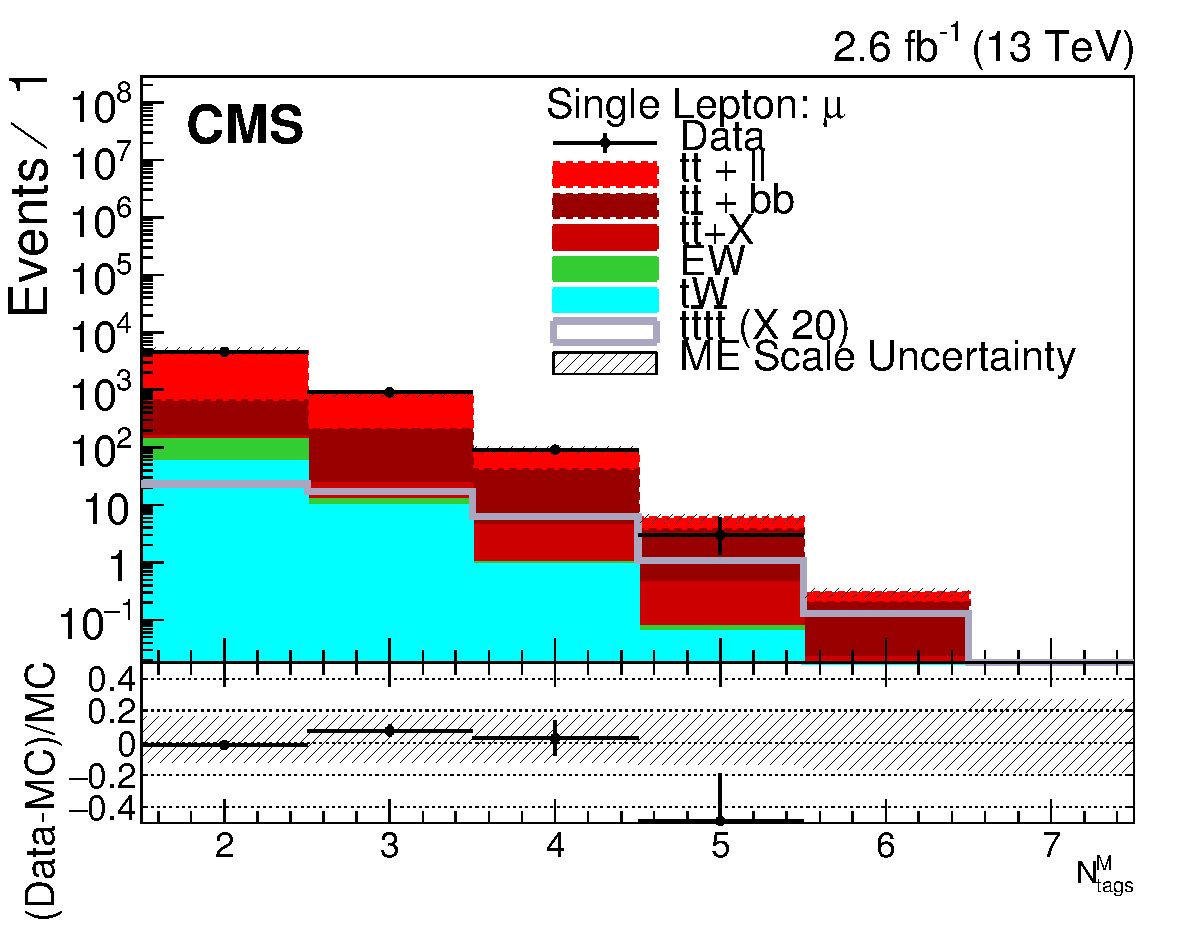
\includegraphics[width=0.47\textwidth]{images/Run2/nMtags_StackLogY_HF_wo_reweight.pdf} 
    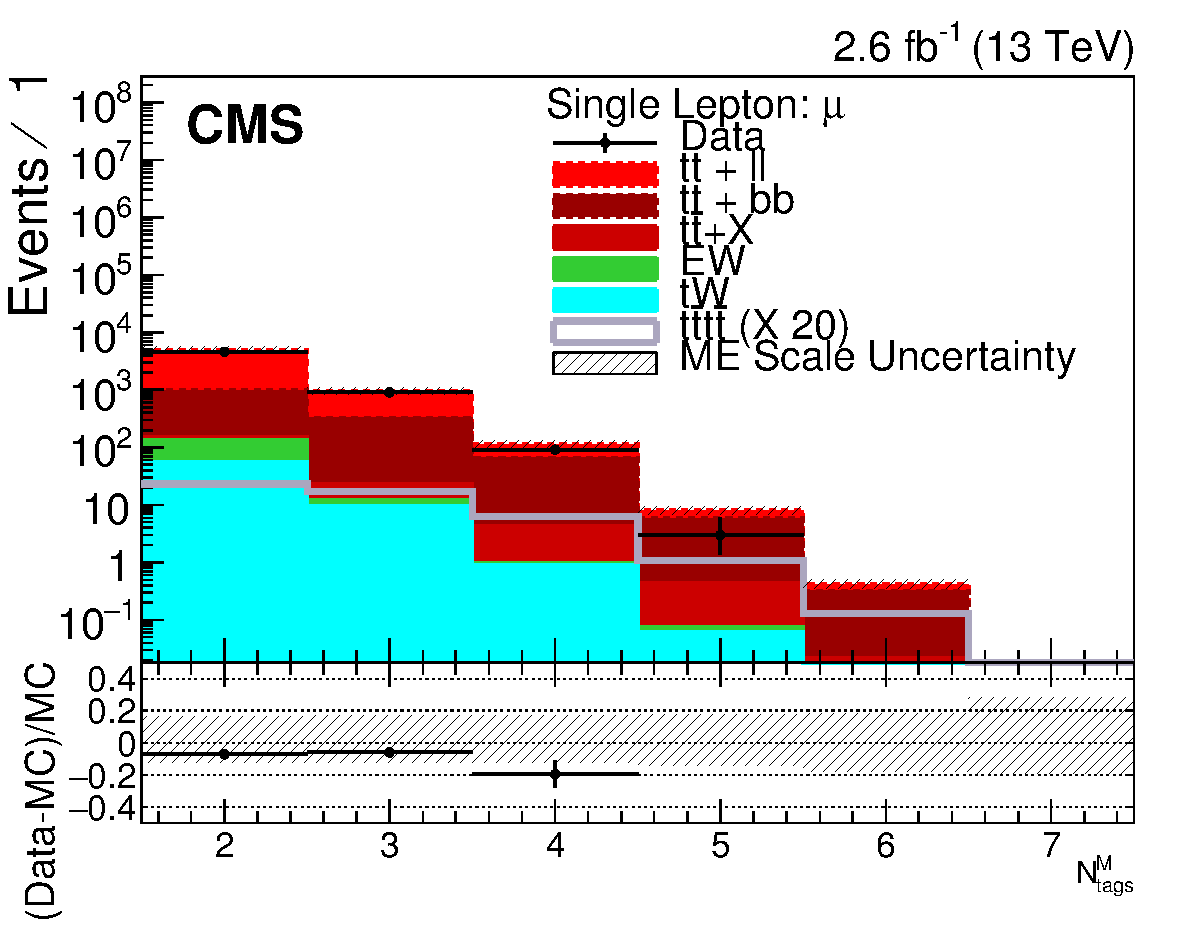
\includegraphics[width=0.47\textwidth]{images/Run2/nMtags_StackLogY_HF_w_reweight.pdf} 
    \caption{\nMtags are shown for the muon channel with heavy flavour reweighting (right) and without(left).}
    \label{fig:HF_reweight}
\end{figure}

\clearpage

\section{Weighted event counts at each baseline event selection requirement \label{cutflow13}}

The event counts, weight by each correction factor in MC, are given after each selection requirement.

\section{Agreement between data and simulation}
Distributions are shown for $HT_{b}$, $HT_{Rat}$, pt$_{trijet1}$, $N_{Ltags}$, $N_{Ttags}$, \redhadmass, HT$_{X}$ and lepton isolation. Good agreement is seen between data and simulation in all distributions with almost all data points within the main ME scale uncertainty represented by the hatched band.

\begin{figure}[ht!]
    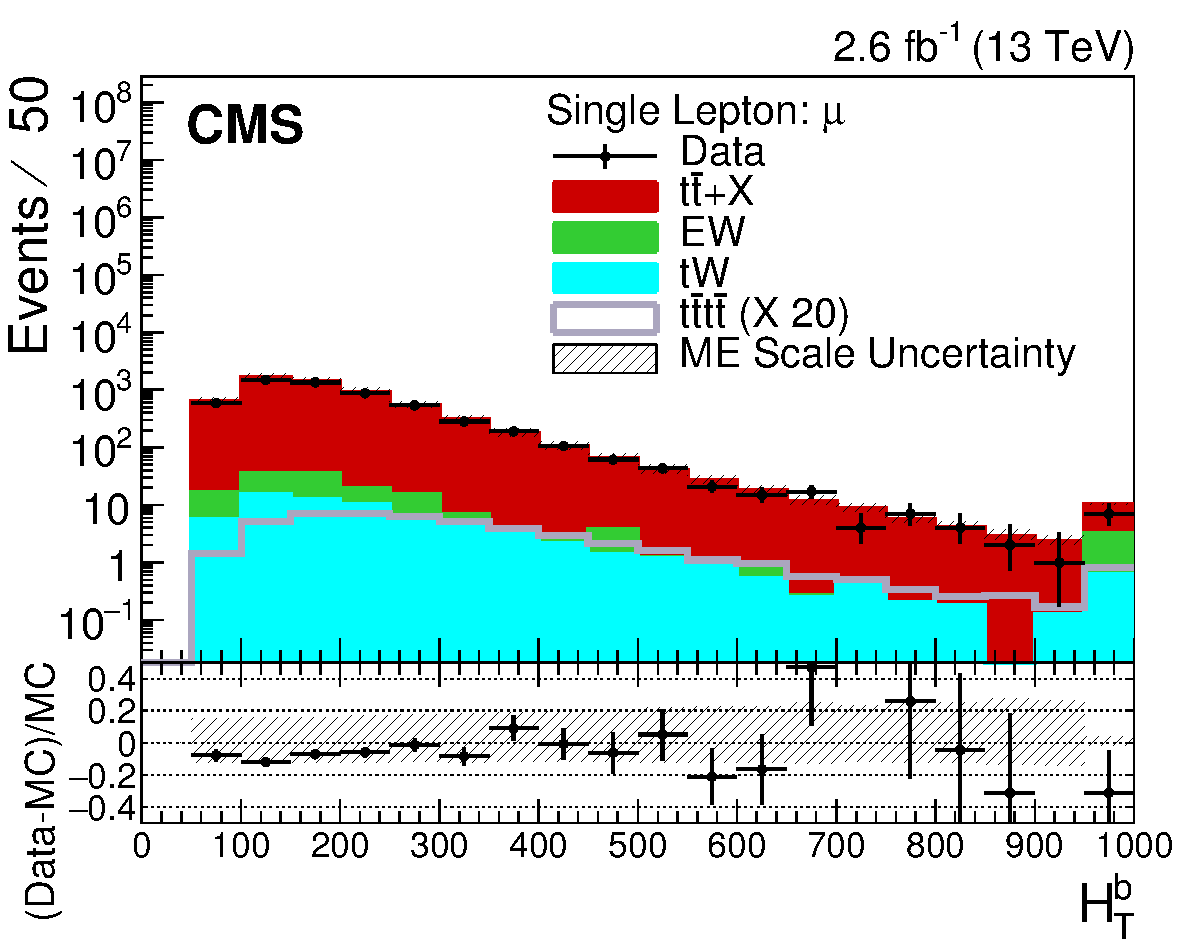
\includegraphics[width=0.48\textwidth]{images/Run2/HTb_StackLogY.pdf}
    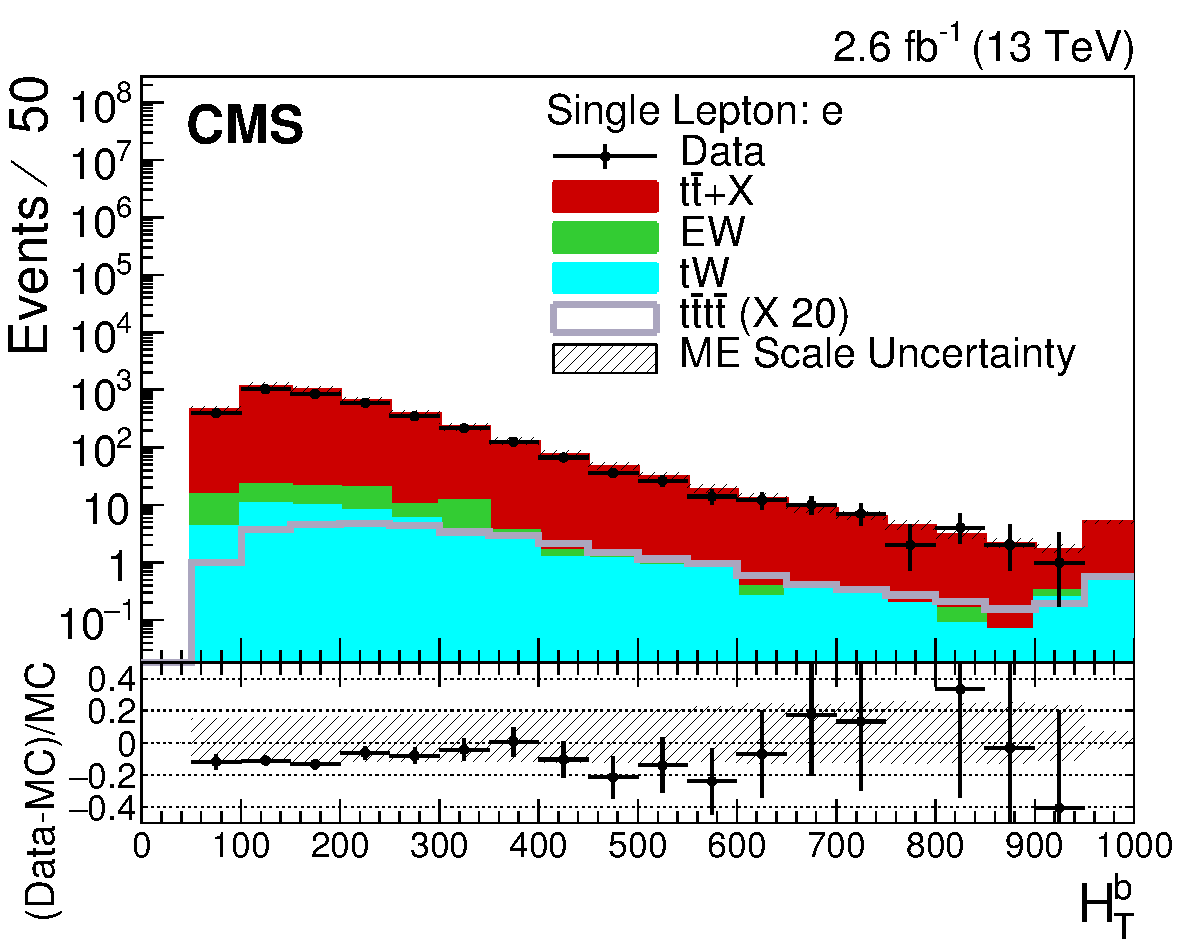
\includegraphics[width=0.48\textwidth]{images/Run2/HTb_StackLogY_e.pdf}
    \caption{The $HT_{b}$ distributions for data and simulation in the $\mu$ + jets channel (left) and $e$ + jets channel (left).}
    \label{fig:HTB}
\end{figure}


\begin{figure}[ht!]
    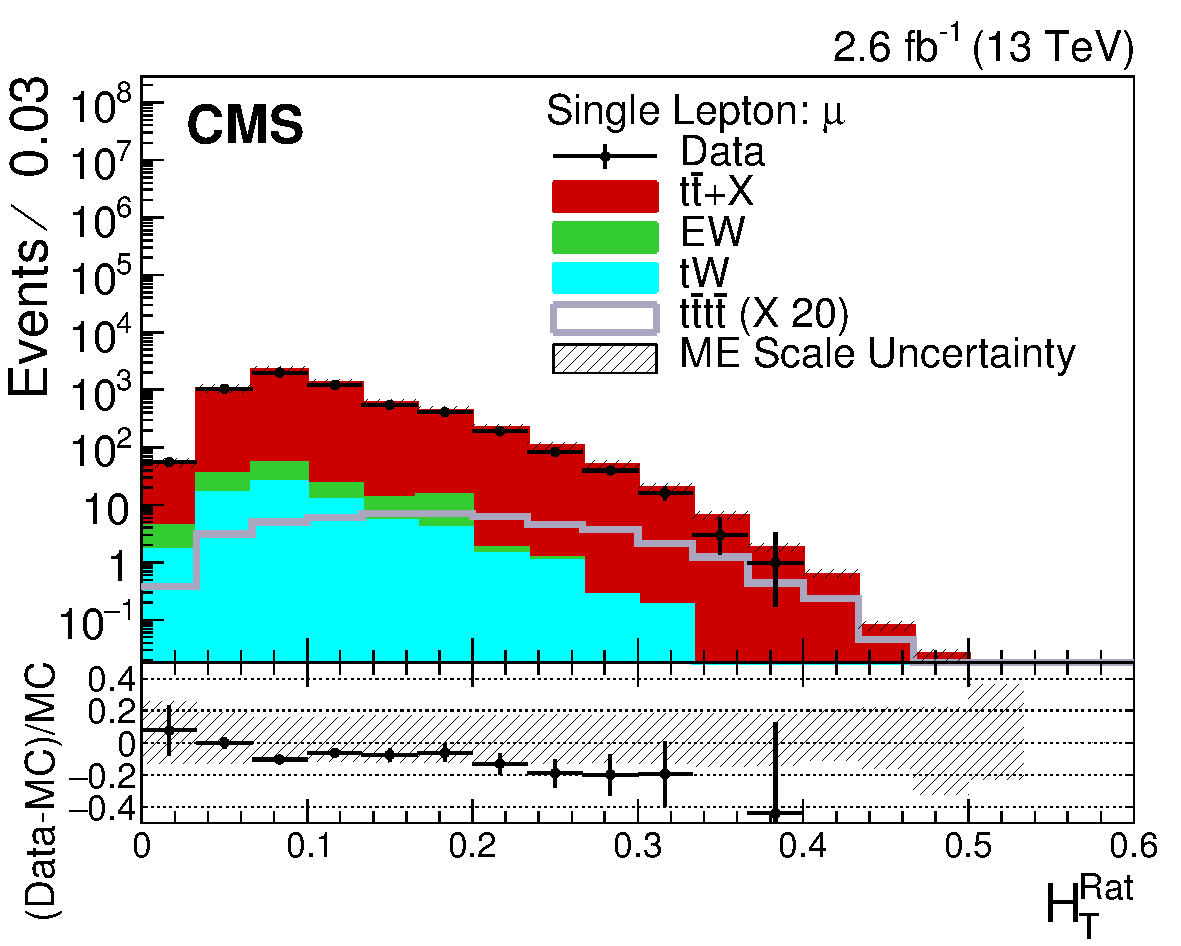
\includegraphics[width=0.48\textwidth]{images/Run2/HTRat_StackLogY.pdf}
    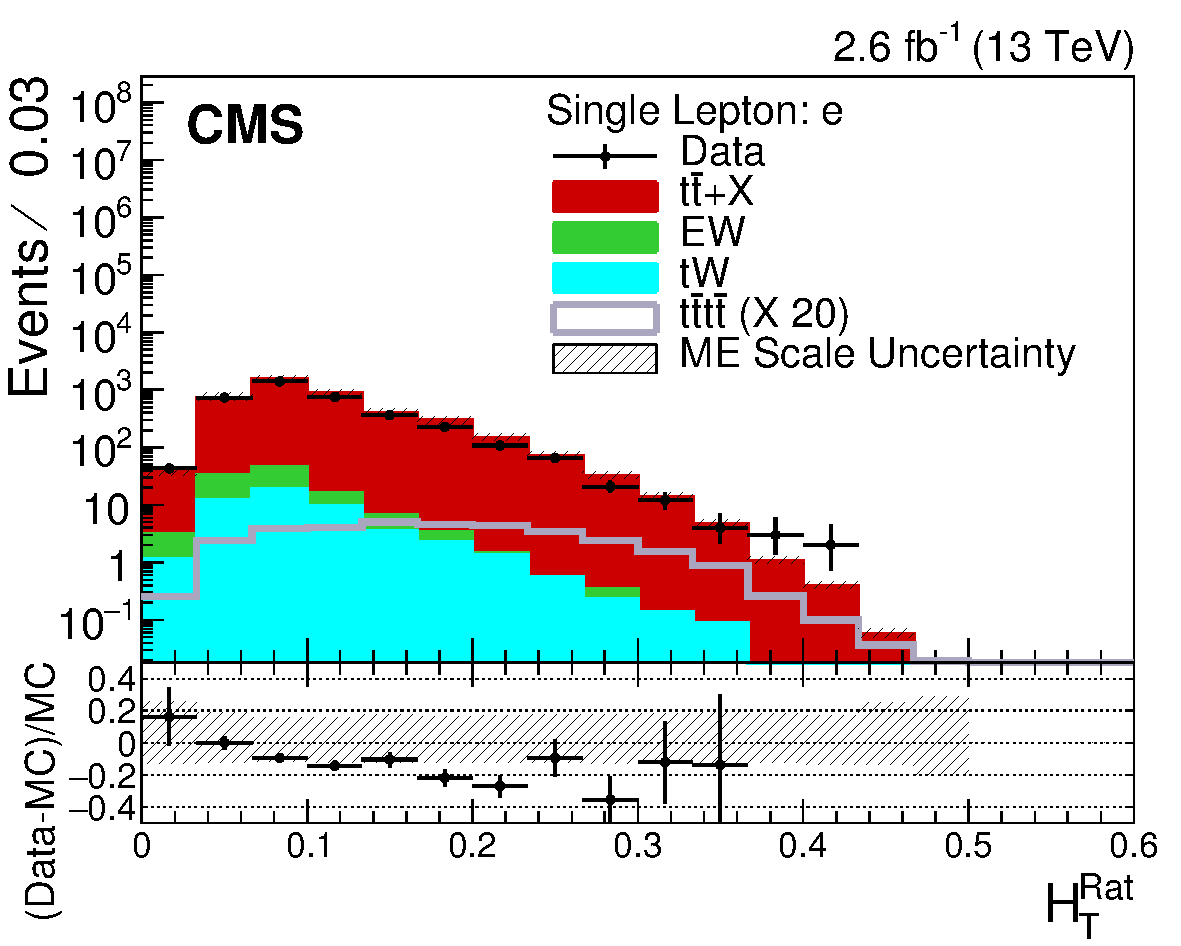
\includegraphics[width=0.48\textwidth]{images/Run2/HTRat_StackLogY_e.pdf}
    \caption{The $HT_{Rat}$ distributions for data and simulation in the $\mu$ + jets channel (left) and $e$ + jets channel (left).}
    \label{fig:HTRat}
\end{figure}



% \begin{figure}[ht!]
%     \includegraphics[width=0.48\textwidth]{images/Run2/LeadingBJetPt_StackLogY.pdf}
%     \includegraphics[width=0.48\textwidth]{images/Run2/LeadingBJetPt_StackLogY.pdf}
%     \caption{The \leadbpt distributions for data and simulation in the $\mu$ + jets channel (left) and $e$ + jets channel (left).}
%     \label{fig:LeadingBJetPt}
% \end{figure}

    
\begin{figure}[ht!]
    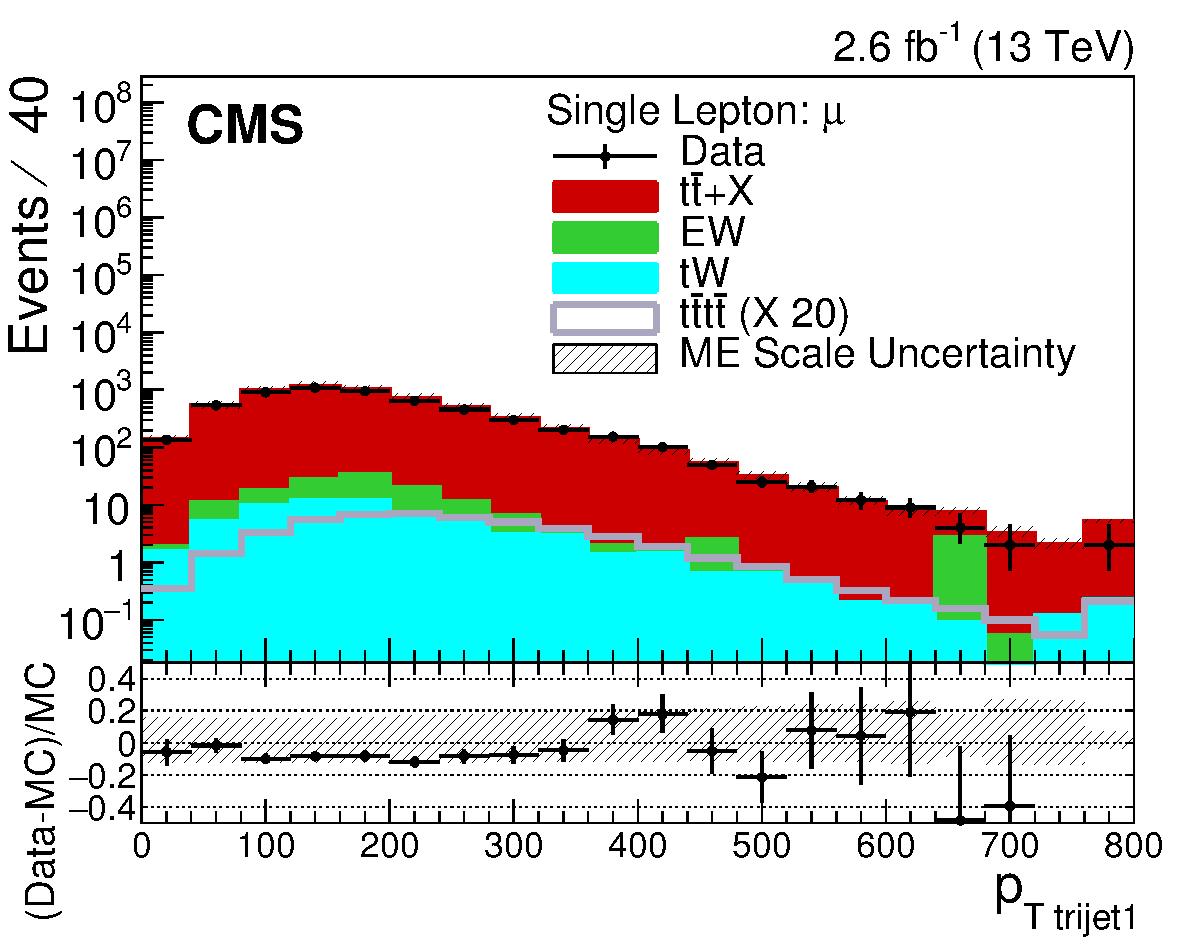
\includegraphics[width=0.48\textwidth]{images/Run2/bestTopPt_StackLogY.pdf}
    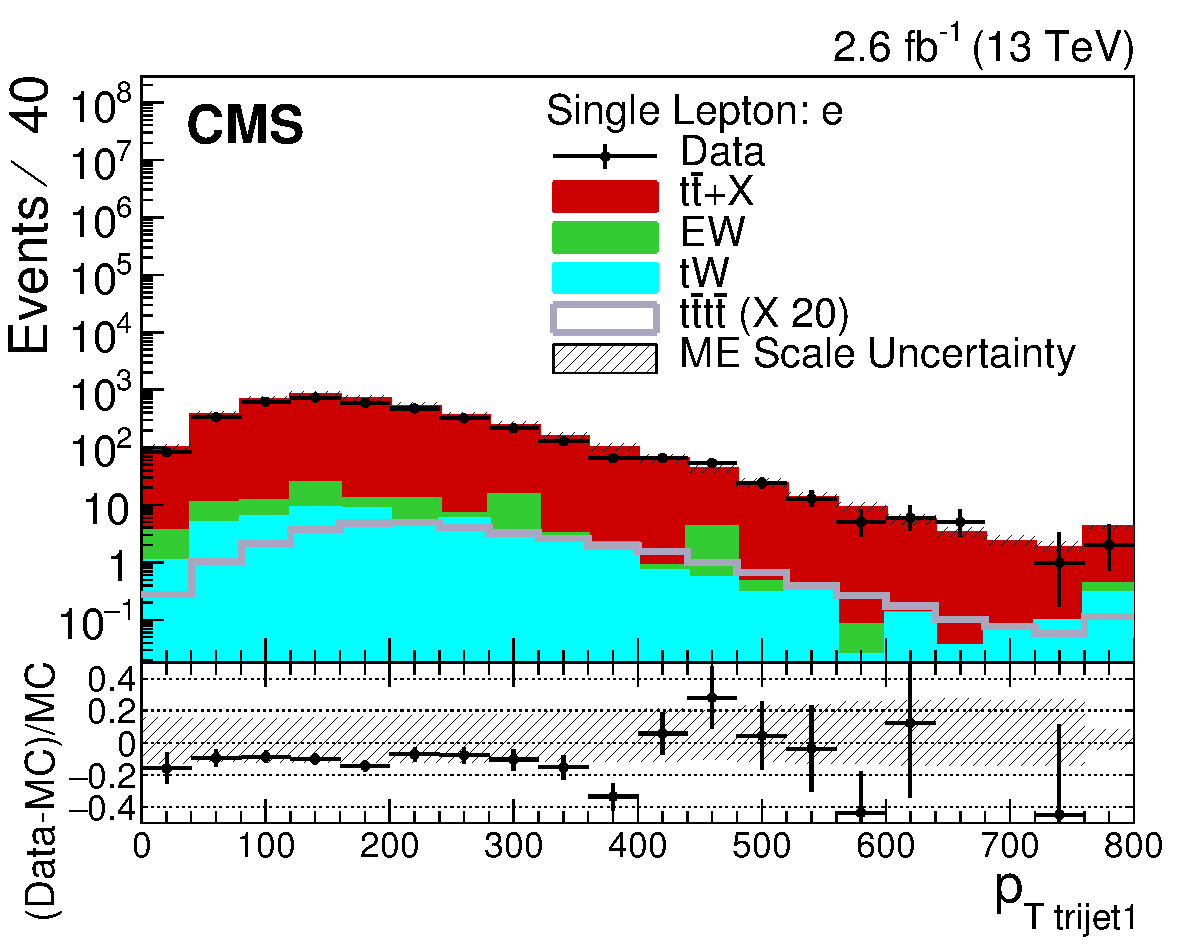
\includegraphics[width=0.48\textwidth]{images/Run2/bestTopPt_StackLogY_e.pdf}
    \caption{The pt$_{trijet1}$ distributions for data and simulation in the $\mu$ + jets channel (left) and $e$ + jets channel (left).}
    \label{fig:bestTopPt}
\end{figure}
   

\begin{figure}[ht!]
    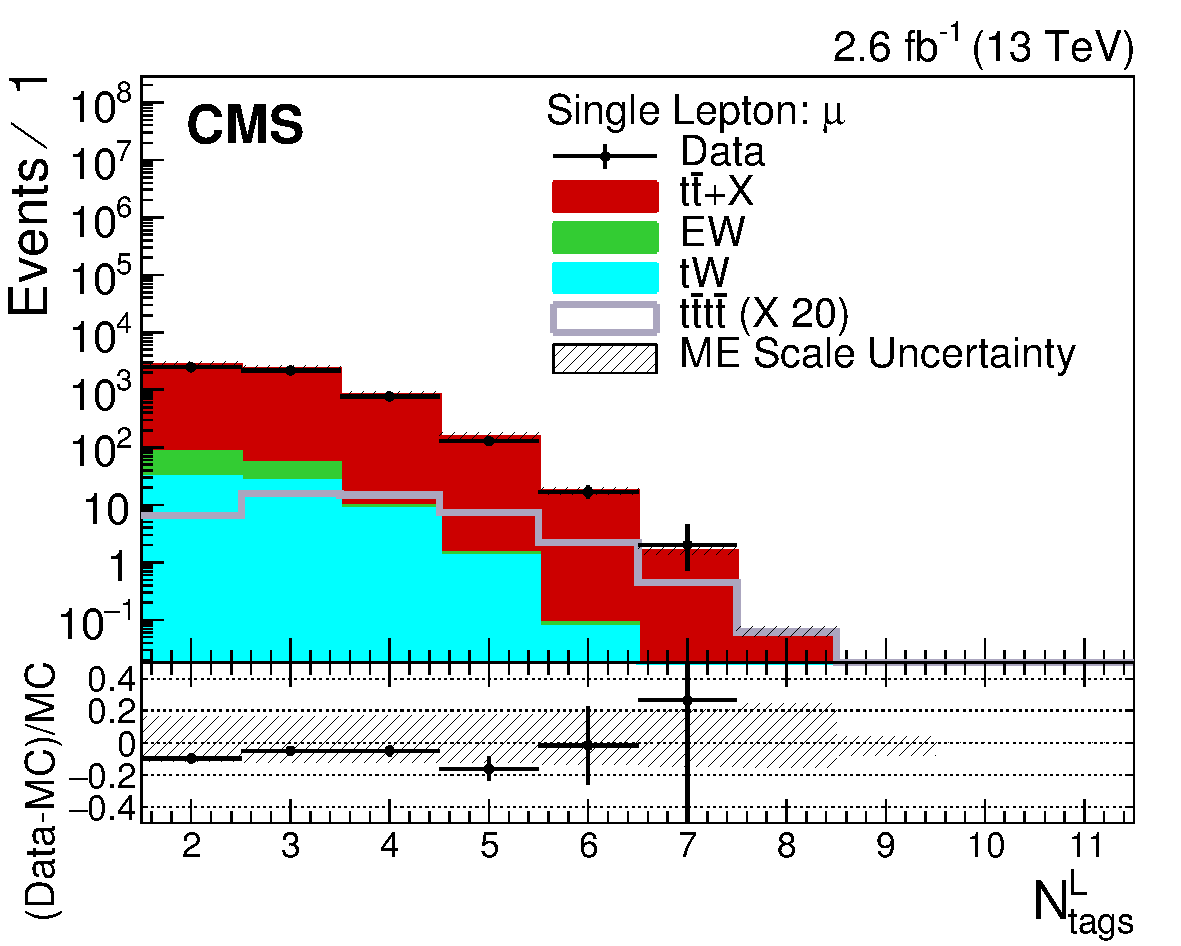
\includegraphics[width=0.48\textwidth]{images/Run2/nLtags_StackLogY.pdf}
    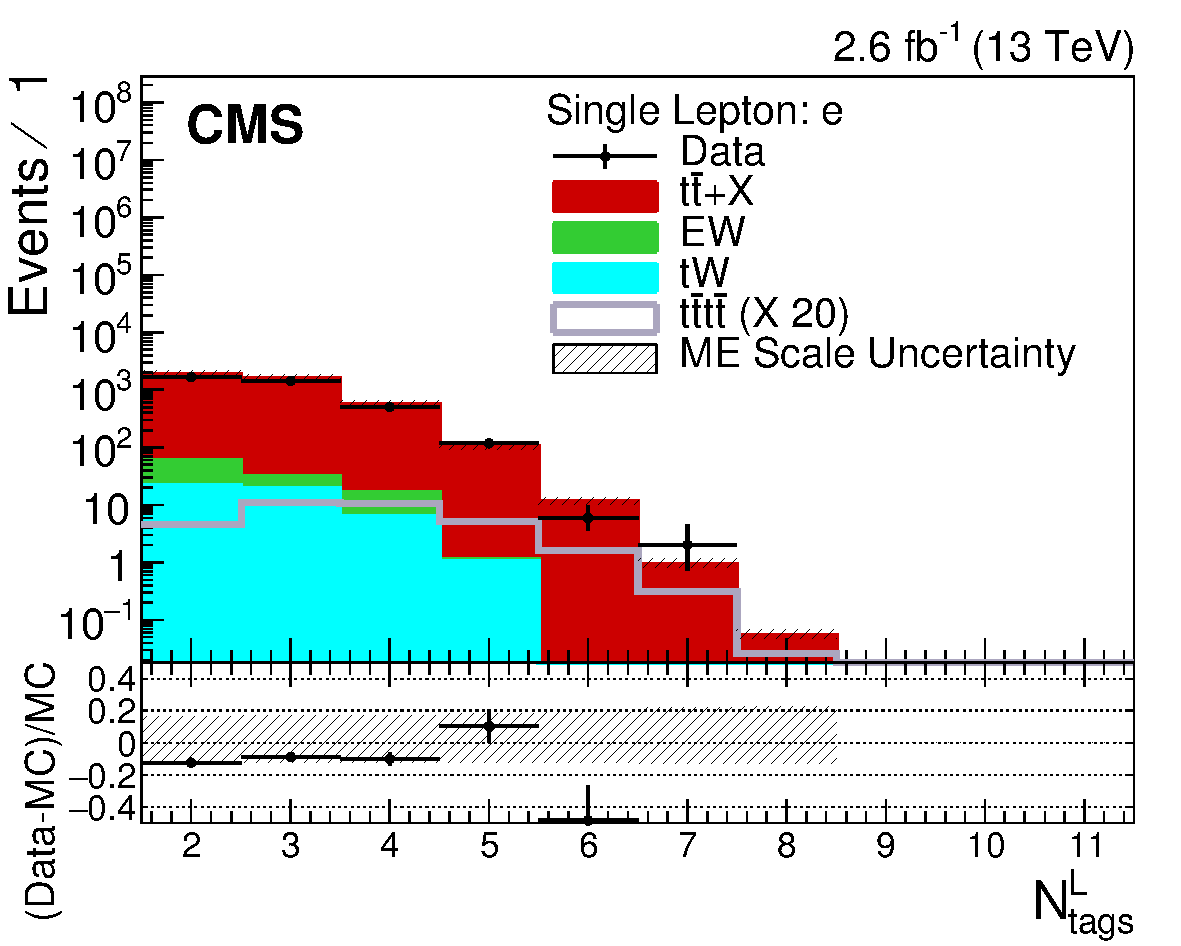
\includegraphics[width=0.48\textwidth]{images/Run2/nLtags_StackLogY_e.pdf}
    \caption{The $N_{Ltags}$ distributions for data and simulation in the $\mu$ + jets channel (left) and $e$ + jets channel (left).}
    \label{fig:nLtagsInc}
\end{figure}

\begin{figure}[ht!]
    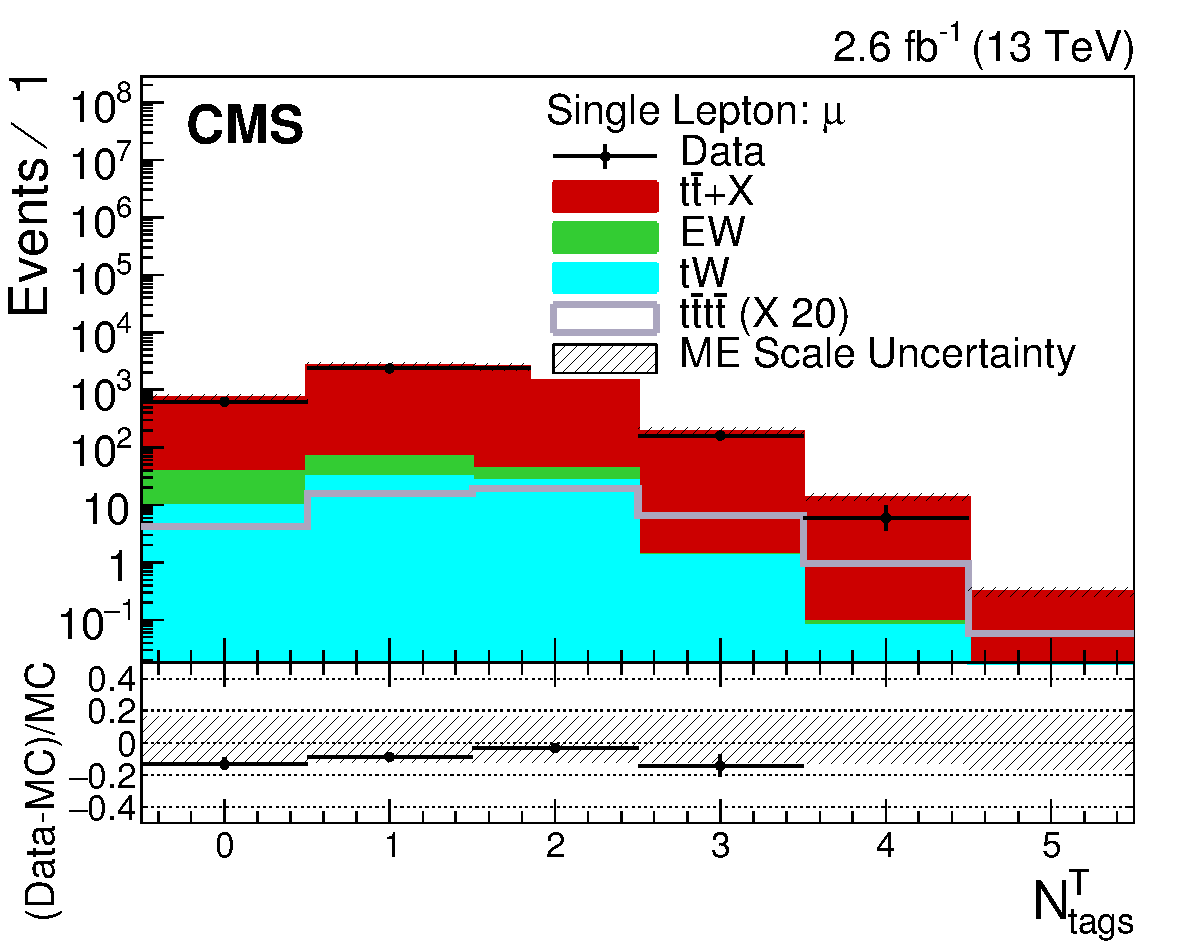
\includegraphics[width=0.48\textwidth]{images/Run2/nTtags_StackLogY.pdf}
    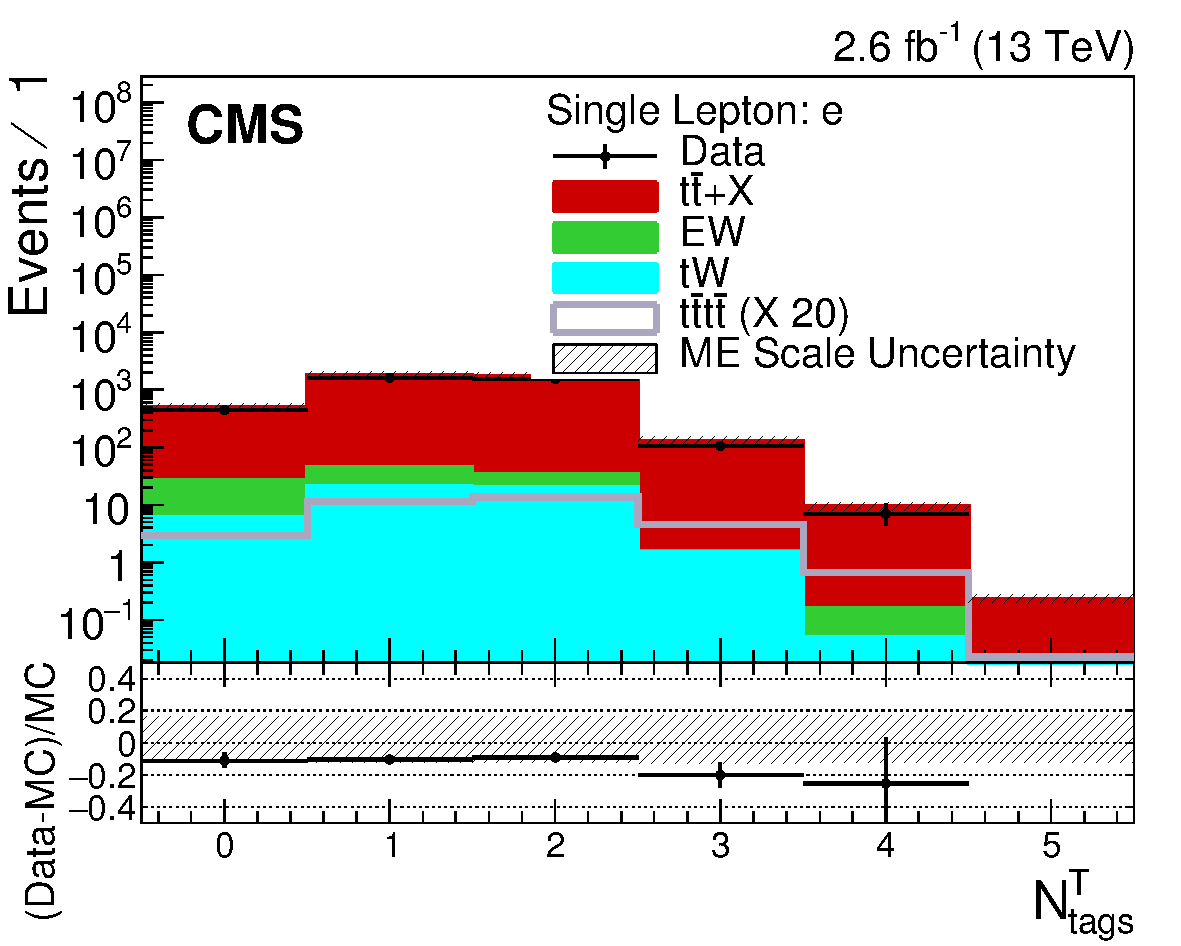
\includegraphics[width=0.48\textwidth]{images/Run2/nTtags_StackLogY_e.pdf}
    \caption{The $N_{Ttags}$ distributions for data and simulation in the $\mu$ + jets channel (left) and $e$ + jets channel (left).}
    \label{fig:nTtagsInc}
\end{figure}

\begin{figure}[ht!]
    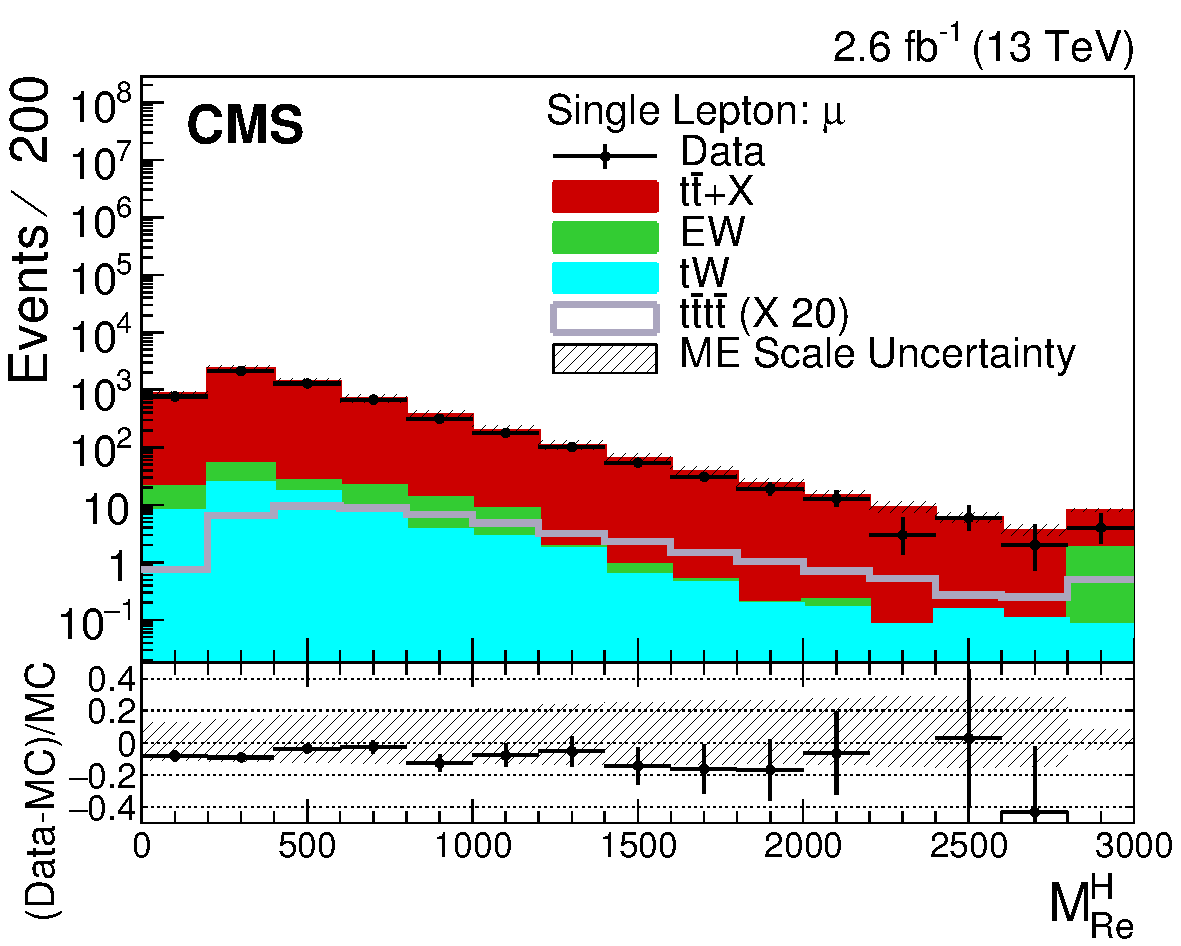
\includegraphics[width=0.48\textwidth]{images/Run2/SumJetMassX_StackLogY.pdf}
    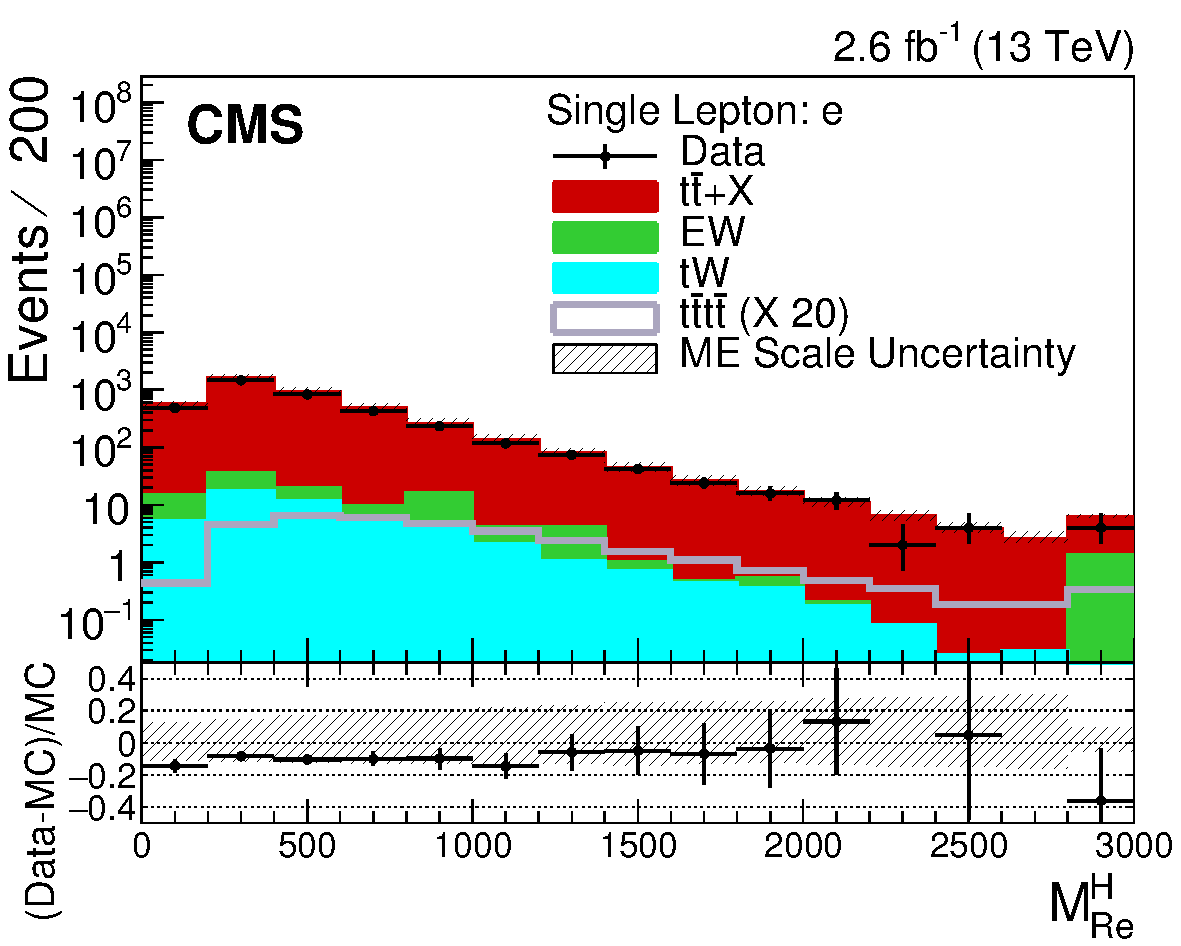
\includegraphics[width=0.48\textwidth]{images/Run2/SumJetMassX_StackLogY_e.pdf}
    \caption{The \redhadmass distributions for data and simulation in the $\mu$ + jets channel (left) and $e$ + jets channel (left).}
    \label{fig:SumJetMassX}
\end{figure}

\begin{figure}[ht!]
    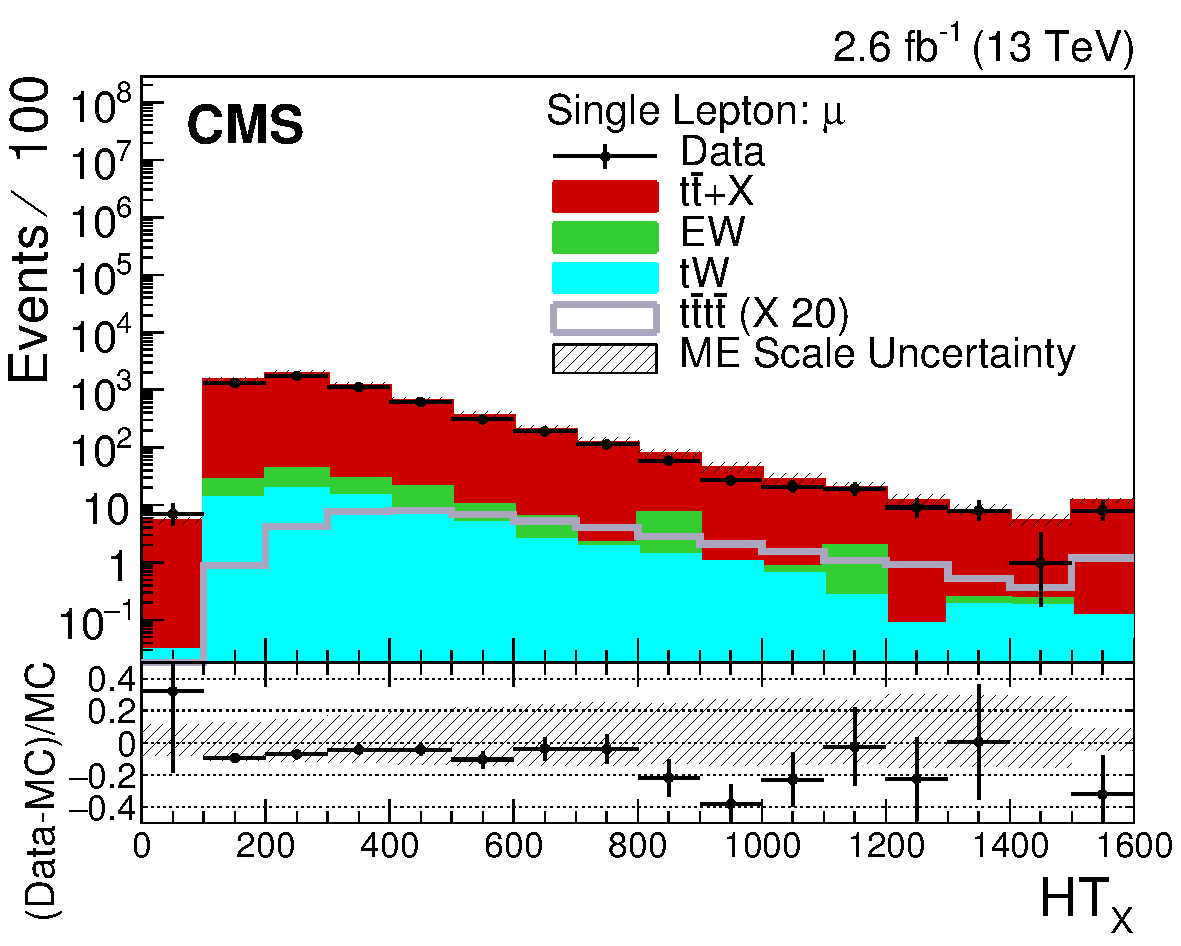
\includegraphics[width=0.48\textwidth]{images/Run2/HTX_StackLogY.pdf}
    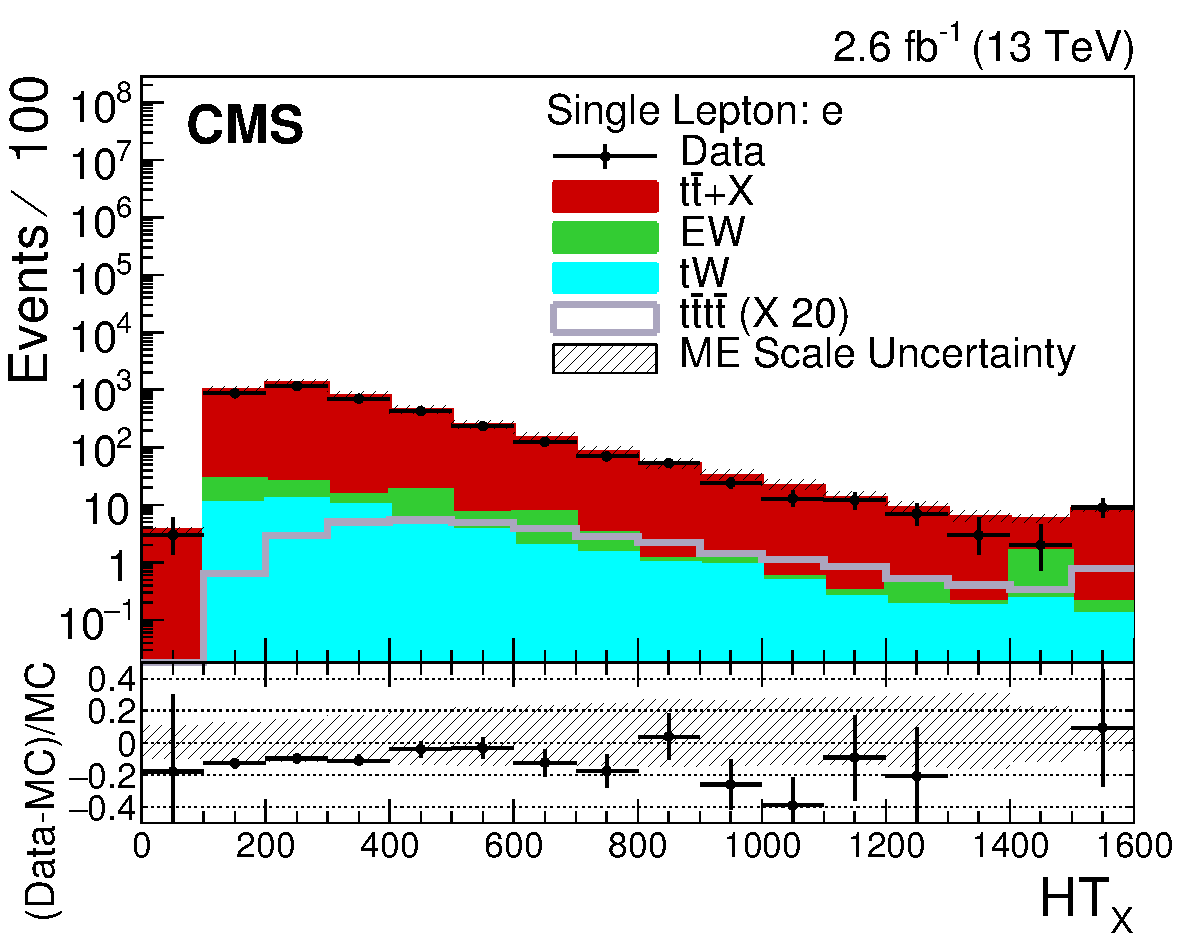
\includegraphics[width=0.48\textwidth]{images/Run2/HTX_StackLogY_e.pdf}
    \caption{The HT$_{X}$ distributions for data and simulation in the $\mu$ + jets channel (left) and $e$ + jets channel (left).}
    \label{fig:HTX}
\end{figure} 

\begin{figure}
    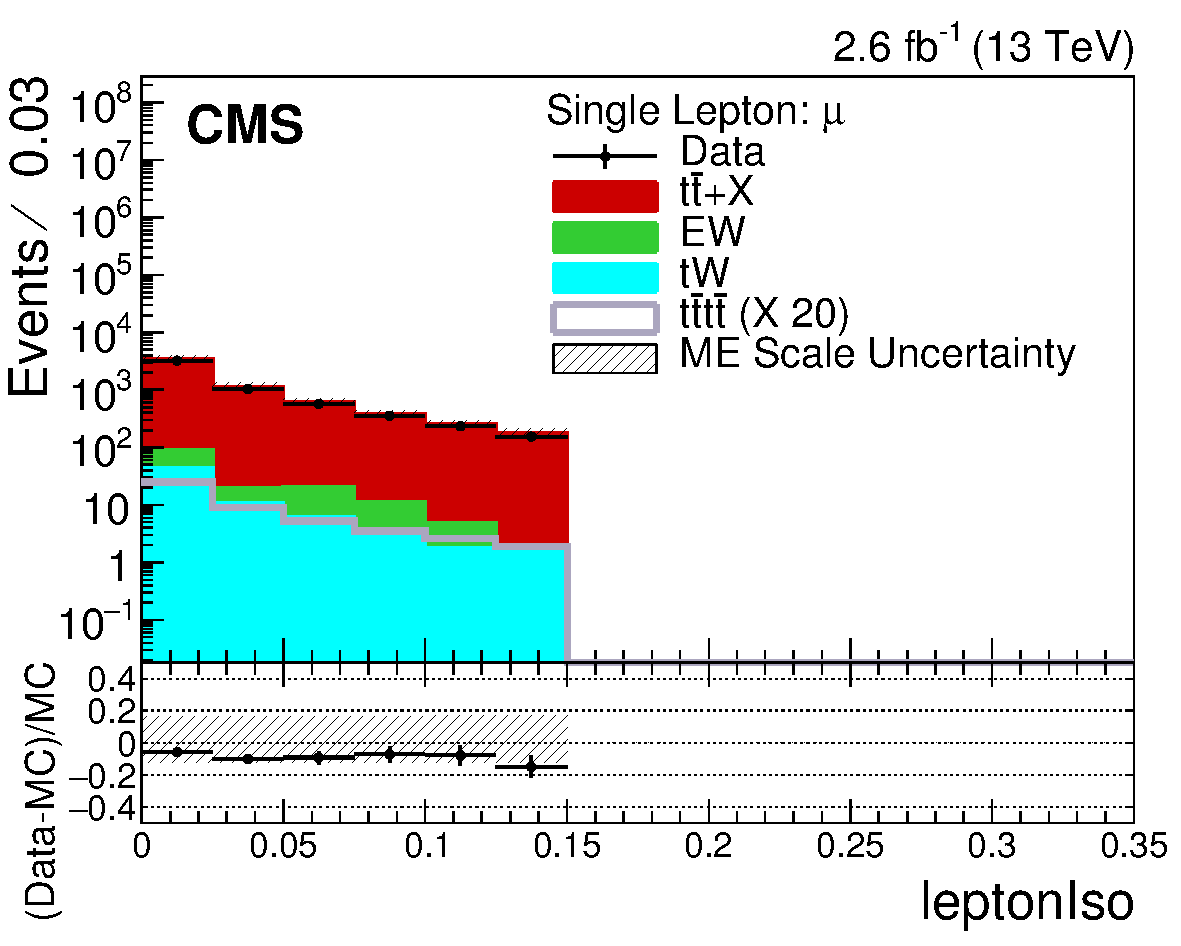
\includegraphics[width=0.48\textwidth]{images/Run2/leptonIso_StackLogY.pdf}
    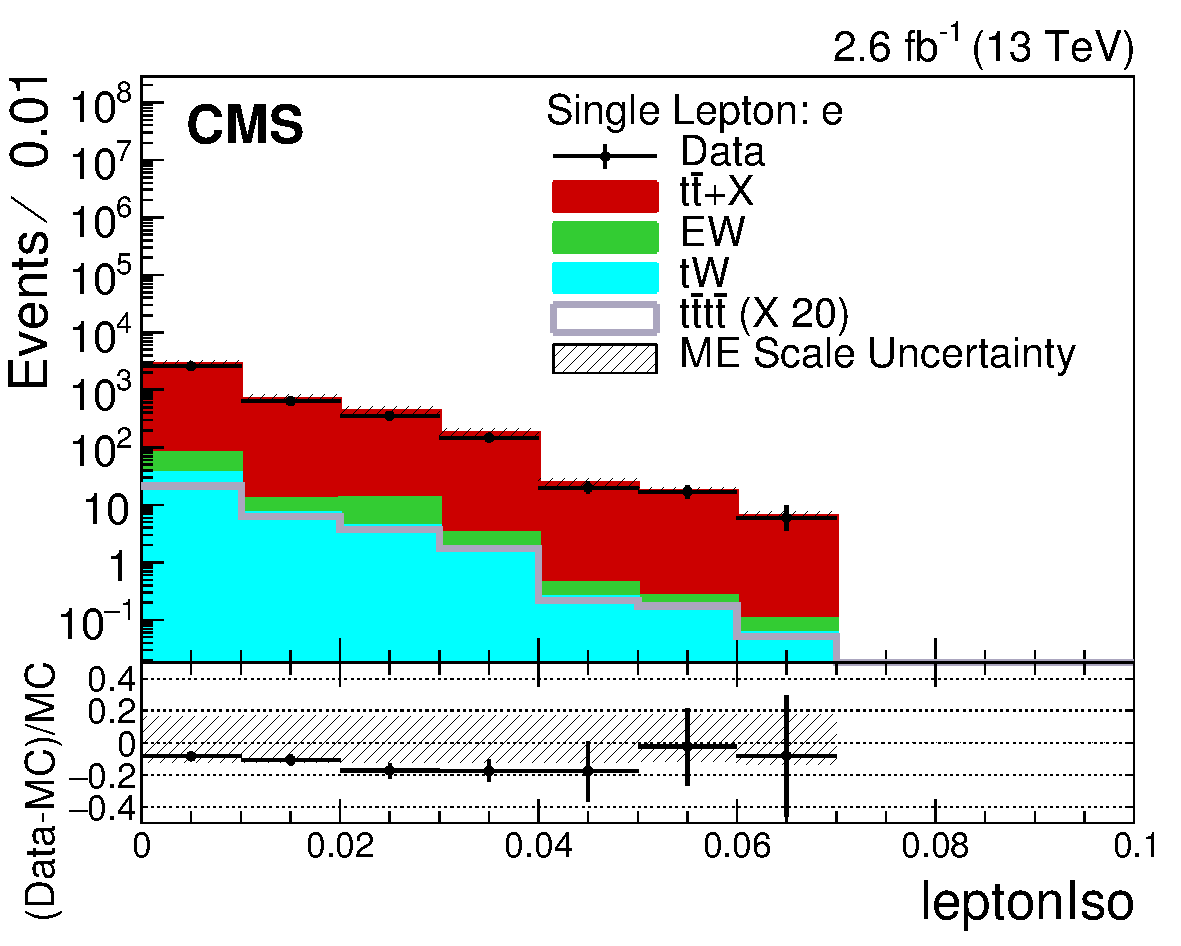
\includegraphics[width=0.48\textwidth]{images/Run2/leptonIso_StackLogY_e.pdf}
    \caption{The lepton isolation distributions for data and simulation in the $\mu$ + jets channel (left) and $e$ + jets channel (left).}
    \label{fig:lepiso}
\end{figure}
\pagebreak

\section{Discriminating between signal and background}
\label{sec:discriminating13}
It can be seen in Section~\ref{cutflow13} that the \ttbar background is three orders of magnitude larger in the signal region. The variables used to discriminate between \ttbar and \tttt are described below.
% There are three main features which can be used to discriminate; the number of top quarks which can be reconstructed in the event, the number of b-jets found in each event, and event activity such as \HT.

\subsection{Hadronic top quark content}
\label{sec:topContent13}

As the \antikt algorithm cannot resolve jets which have $\Delta R = \sqrt{  \theta^{2} + \phi^{2} } < 0.4$, a hadronically decaying top quark can only be deemed \emph{reconstructible} if the minimal $\Delta R$ between all three jets is $> 0.4$ which happens $> 98\%$ of the time in \ttbar and \tttt simulation when studying the decay products of leptons and partons, and pairs of partons.\\
The BDT training was performed on 273~K \ttbar events. The input variables to the hadronic top quark reconstruction BDT are shown in Fig.~\ref{fig:TrijetBDTInputFeatures13}. The separation power for each of these variables and for the output BDT discriminator distribution in Fig.~\ref{fig:TrijetBDTOutput13} is evident as in the \runone studies in Chapter~\ref{c:Run1}. 

\begin{figure}[ht!]
\centering
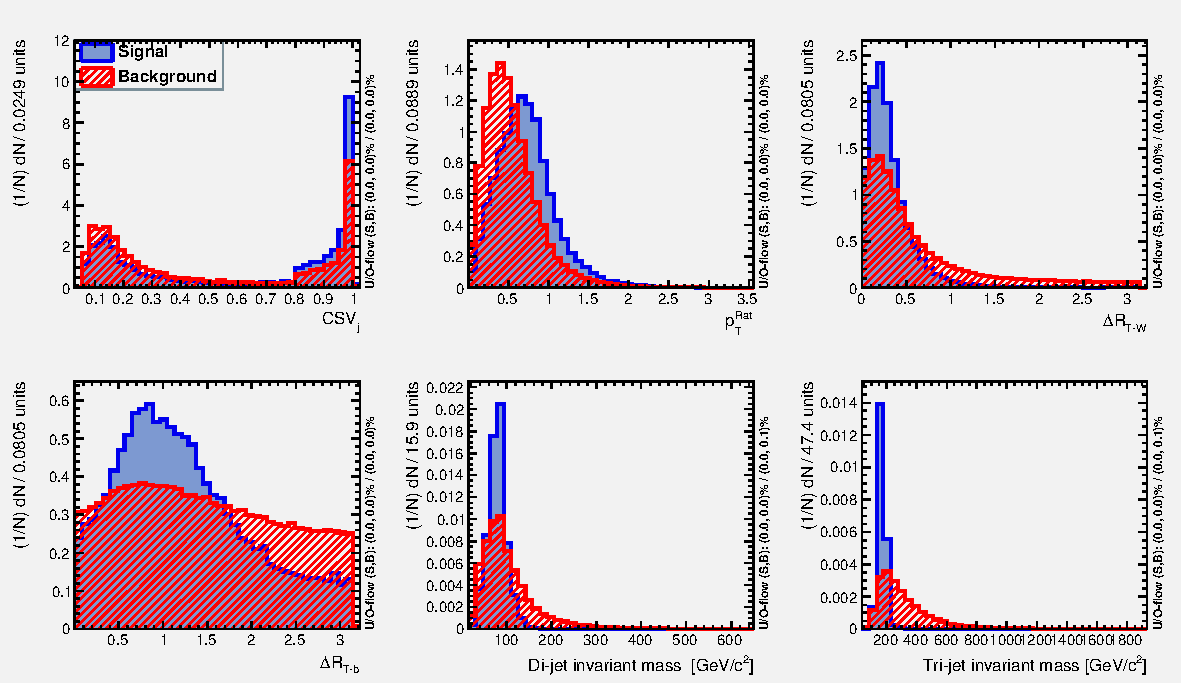
\includegraphics[width=\linewidth]{images/Run2/variables_id_c1.pdf}
\caption{Normalised distributions of the six variables used the MVA hadronic Top kinematic reconstruction are shown for good (red histograms) and bad (blue histograms) trijets.}
\label{fig:TrijetBDTInputFeatures13}
\end{figure}

\begin{figure}[ht!]
\begin{center}
    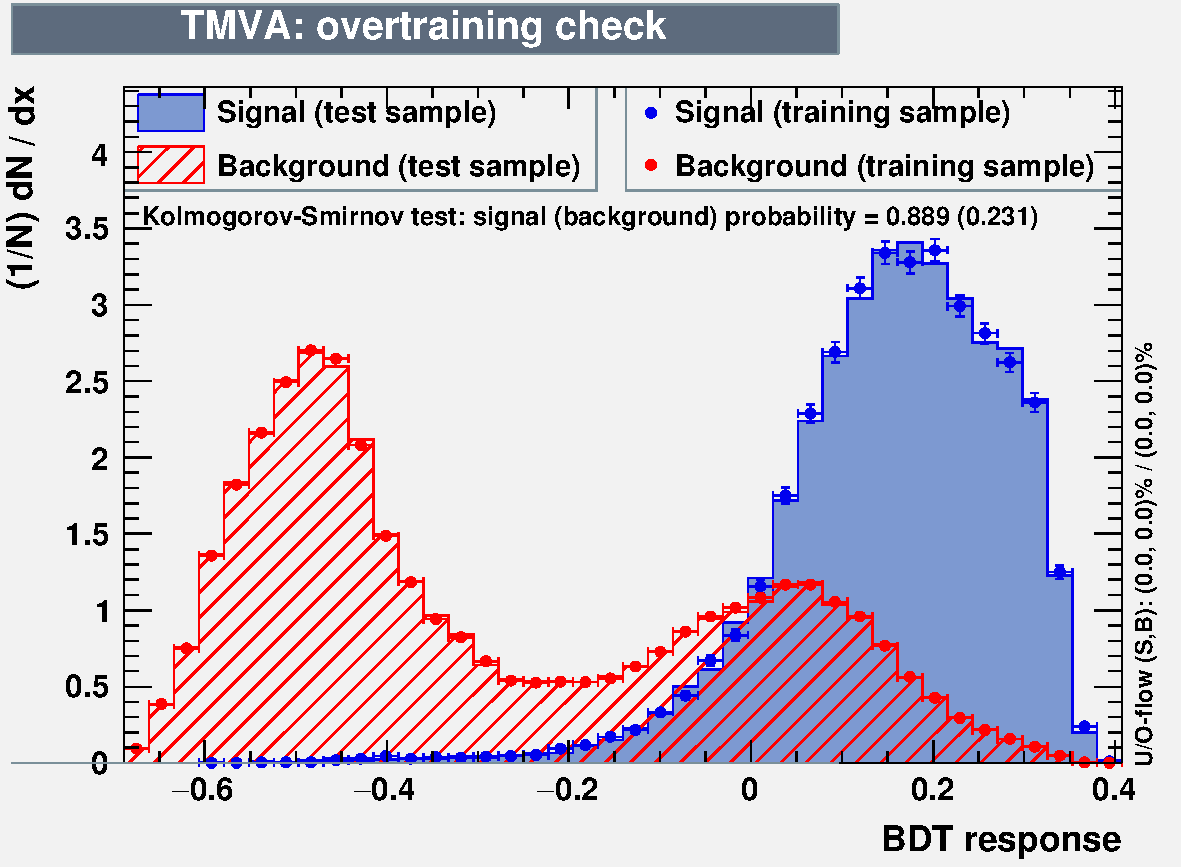
\includegraphics[width=0.55\textwidth]{images/Run2/overtrain_BDT.pdf}
    \caption{The discriminator distributions for the BDT classifier for good (blue) and bad (red) trijets in training and validation samples.}
    \label{fig:TrijetBDTOutput13}
\end{center}
\end{figure}

The affect of the tri-jet invariant mass variable in the BDT is shown in Fig.~\ref{fig:multimode13} where it can be clearly seen that this variable contributes to the strong splitting of the BDT output distribution at a value of $\approx-0.2$.

\begin{figure}[ht!]
\begin{center}
    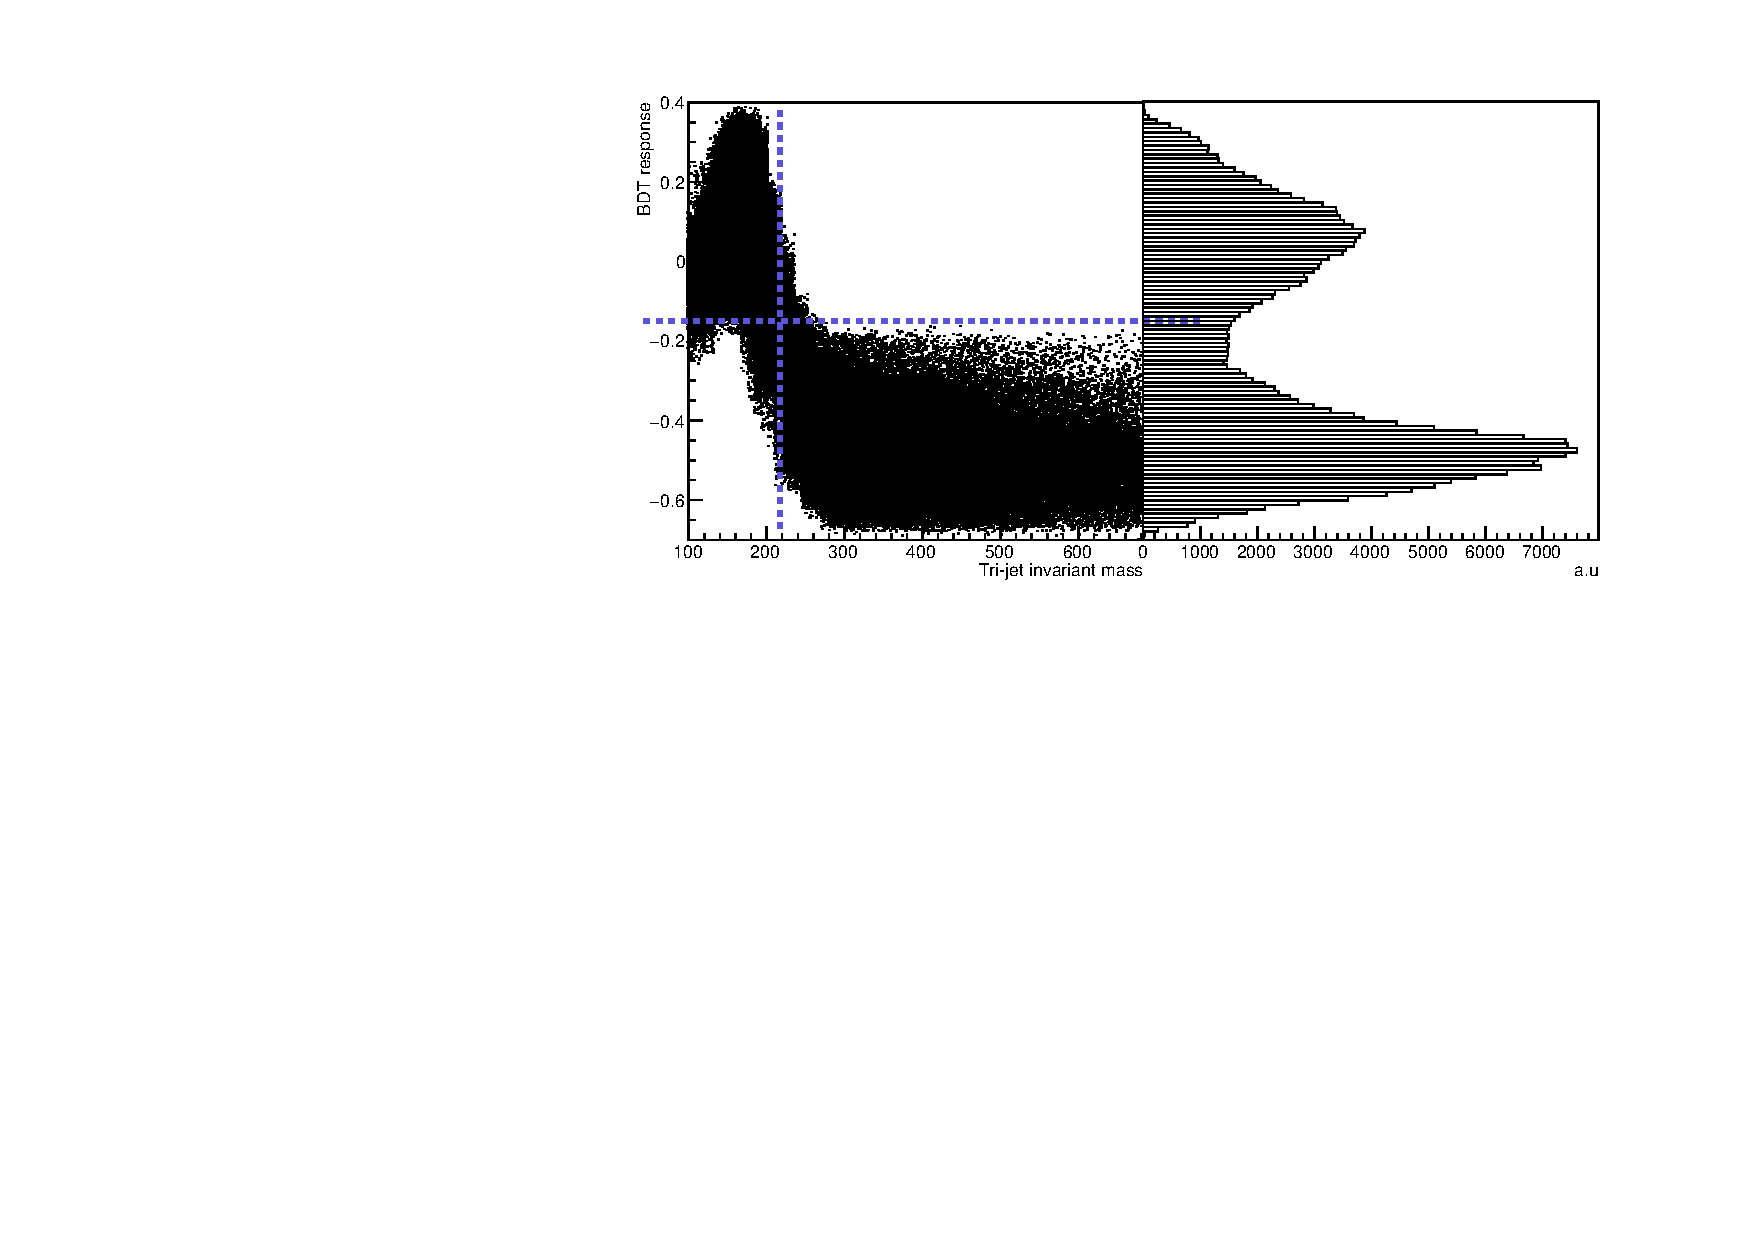
\includegraphics[width=0.85\textwidth]{images/Run2/multimode.pdf}
    \caption{The discriminator distributions for the BDT classifier versus trijet invariant mass and the projection on the vertical axis. Dashed lines indicate the cut value on trijet invariant mass at the BDT root node.}
    \label{fig:multimode13}
\end{center}
\end{figure}

Figure~\ref{fig:ContoursTopMassHadrWmass13}~(left) shows the distribution of good and bad tri-jet combinations in the phase space of tri-jet and di-jet invariant mass. It can be seen from Fig.~\ref{fig:ContoursTopMassHadrWmass13}~(right) that high BDT discriminator values are found in the region where the good tri-jet combinations are clustered.
\begin{figure}[ht!]
\begin{center}
    \includegraphics[width=\textwidth]{images/Run2/ContoursHadrWmassTopMass.pdf}
    \caption{(Left)  Di-jet versus trijet invariant mass distribution for good (blue) and bad (red) trijet combinations. (Right) The average BDT response as a function of Di-jet versus trijet invariant mass input variables.}
    \label{fig:ContoursTopMassHadrWmass13}
\end{center}
\end{figure}

\subsubsection*{BDT$_{tri-jet2}$}

The distribution for BDT$_{tri-jet2}$ is shown in Fig.~\ref{fig:bdtTrijet213}. There is good agreement between the data and simulation and sufficient discrimination power to be used in the event-level BDT.

\begin{figure}[ht!]
    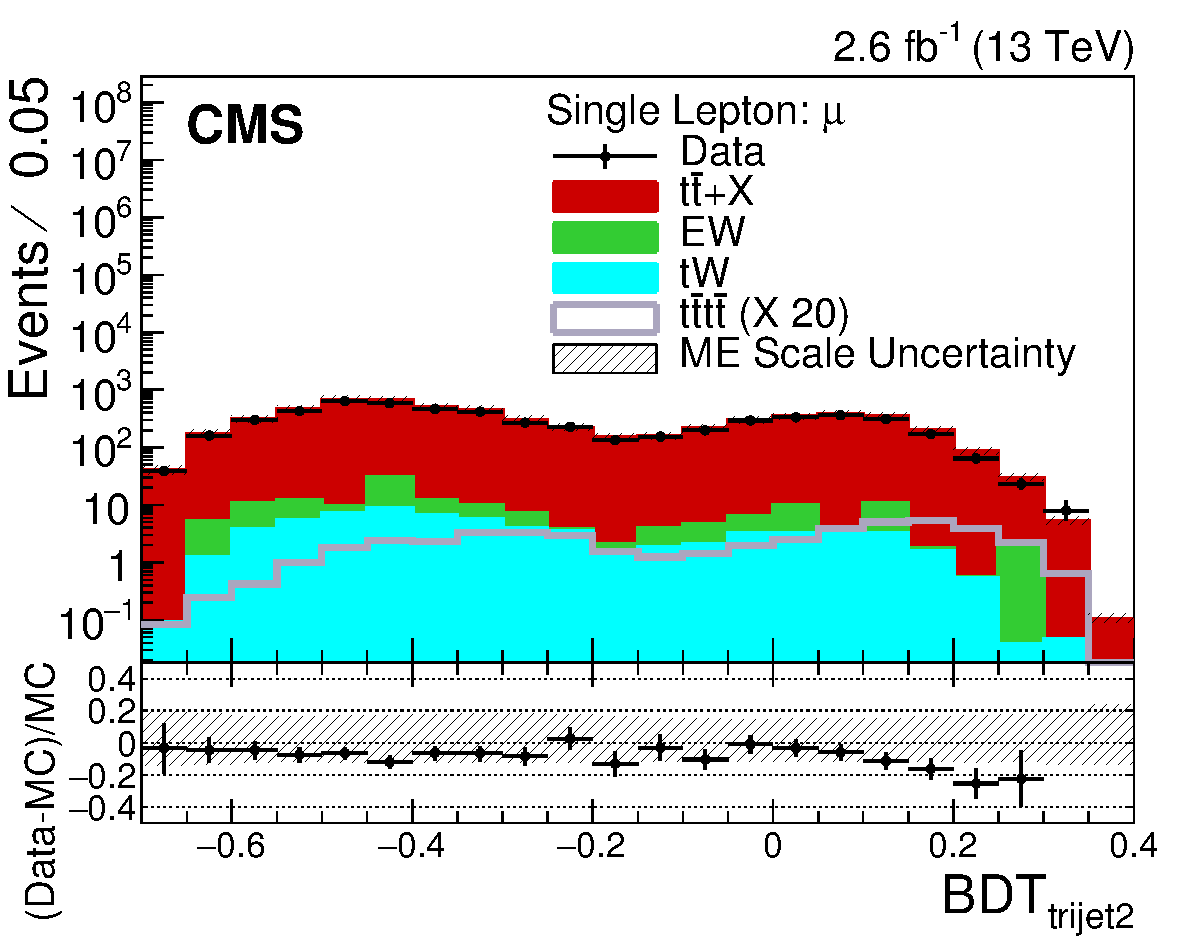
\includegraphics[width=0.44\textwidth]{images/Run2/BDT_trijet2_StackLogY.pdf}
    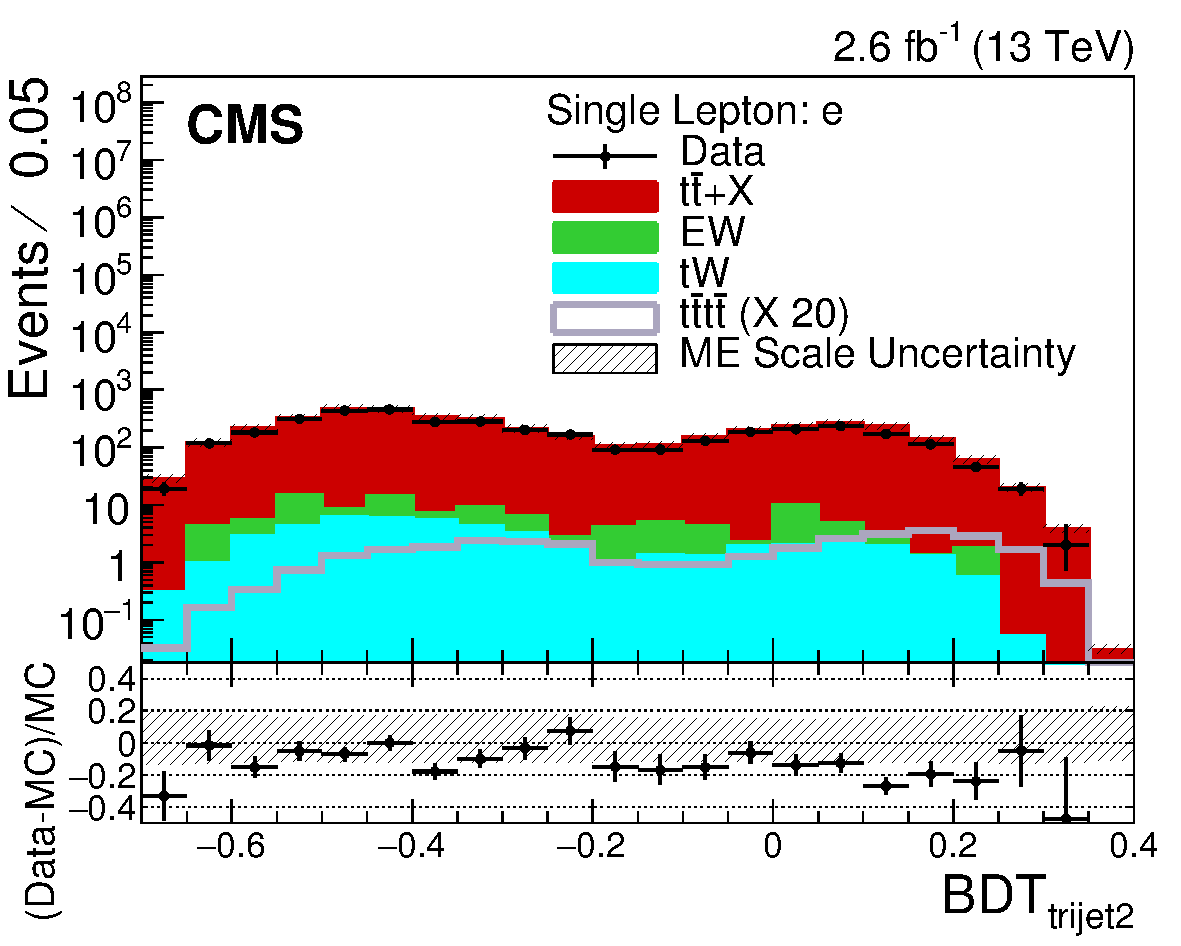
\includegraphics[width=0.44\textwidth]{images/Run2/BDT_trijet2_StackLogY_e.pdf}
    \caption{ The BDT$_{trijet2}$ distributions for data and simulation event in the $\mu$ + jets channel (left) and $e$ + jets channel (right) are plotted.}
    \label{fig:bdtTrijet213}
\end{figure}

\subsubsection*{Reduced Event Variables}
The reduced variables formed from the reduced event, where the jets from the highest-ranked hadronic top quark have been removed from the collection of jets, are shown in Figs.~\ref{fig:htx13} and~\ref{fig:sumjetmassx13}. Again, good agreement is observed between the data and simulation and both variables were found to have good discrimination power in the event-level BDT.

\begin{figure}[ht!]
    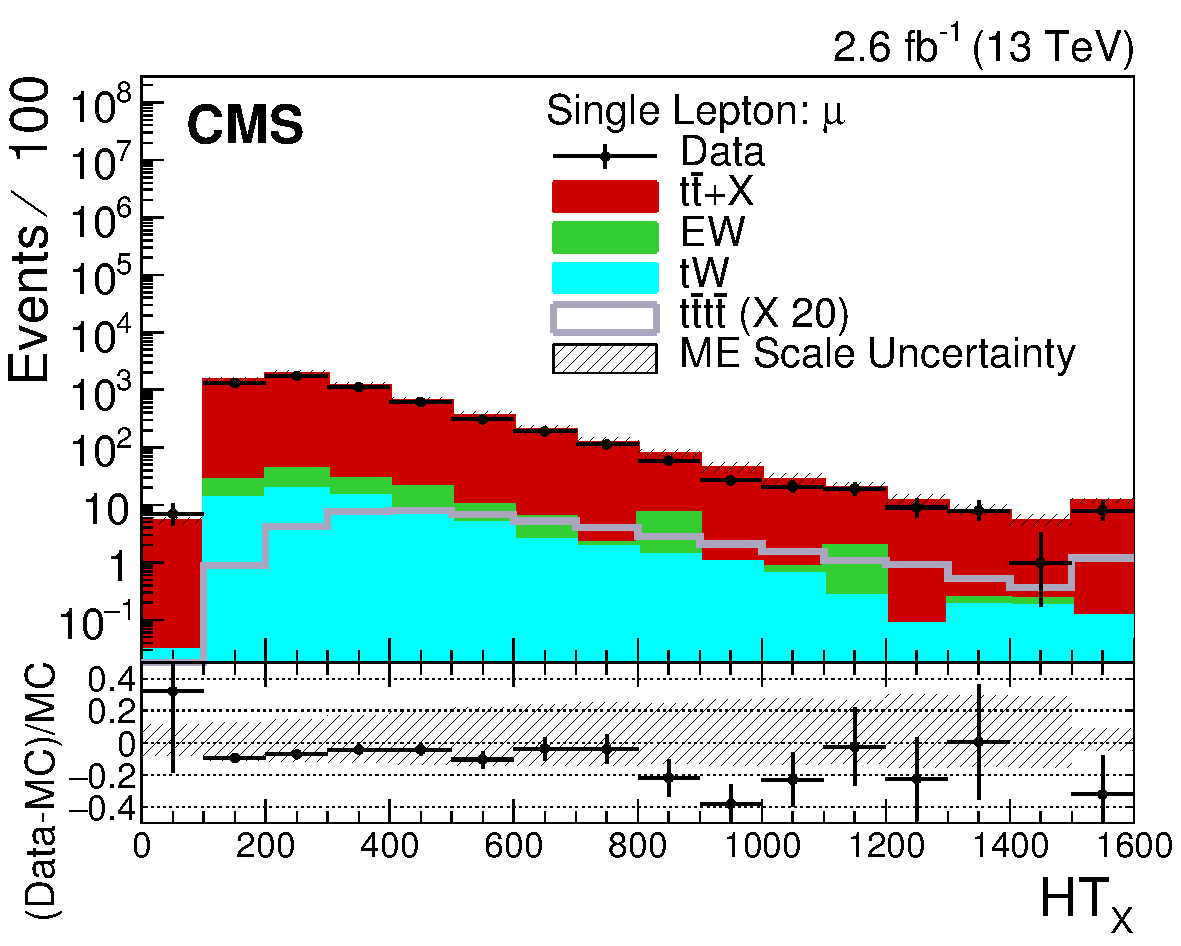
\includegraphics[width=0.44\textwidth]{images/Run2/HTX_StackLogY.pdf}
    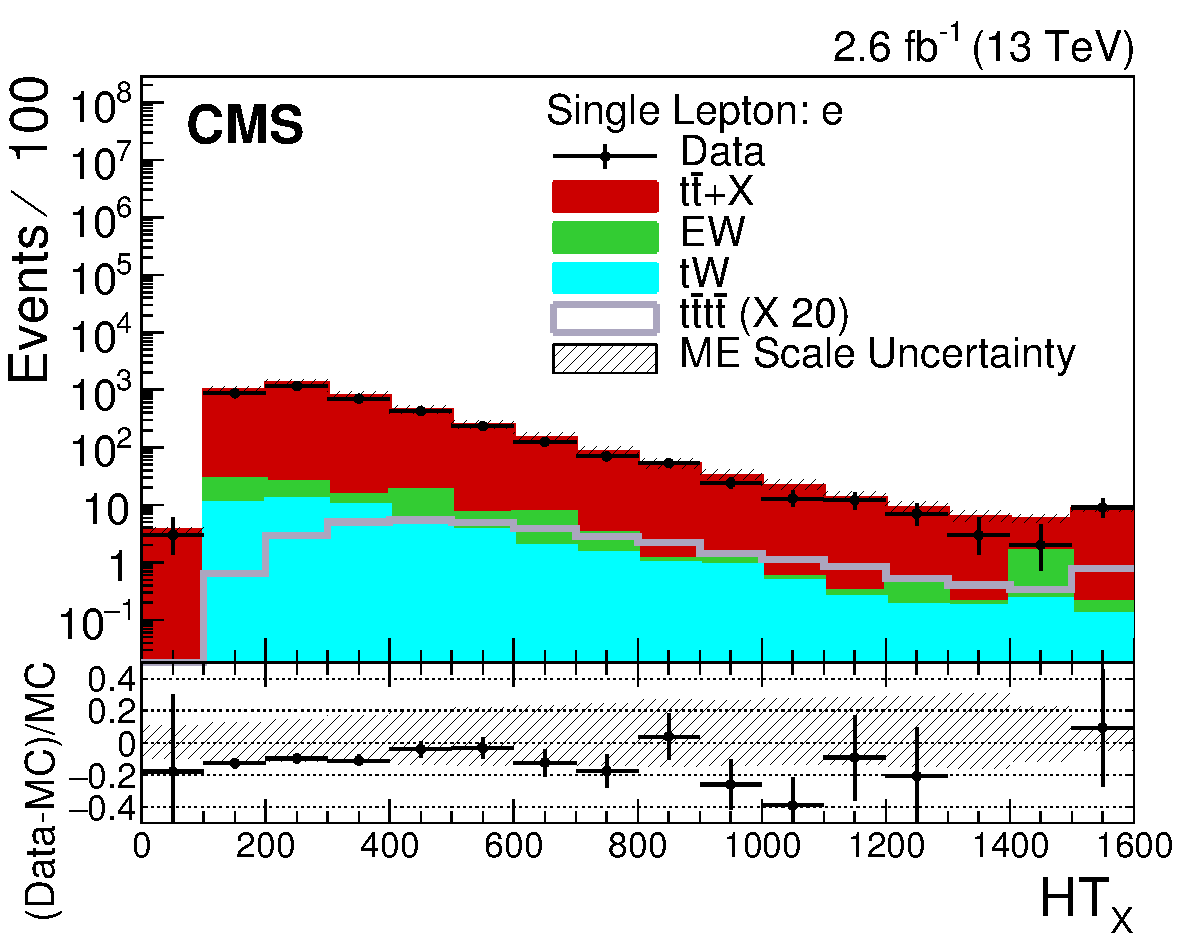
\includegraphics[width=0.44\textwidth]{images/Run2/HTX_StackLogY_e.pdf}
    \caption{ The \HTX distributions for data and simulation event in the $\mu$ + jets channel (left) and $e$ + jets channel (right) are plotted.}
    \label{fig:htx13}
\end{figure}

\begin{figure}[ht!]
    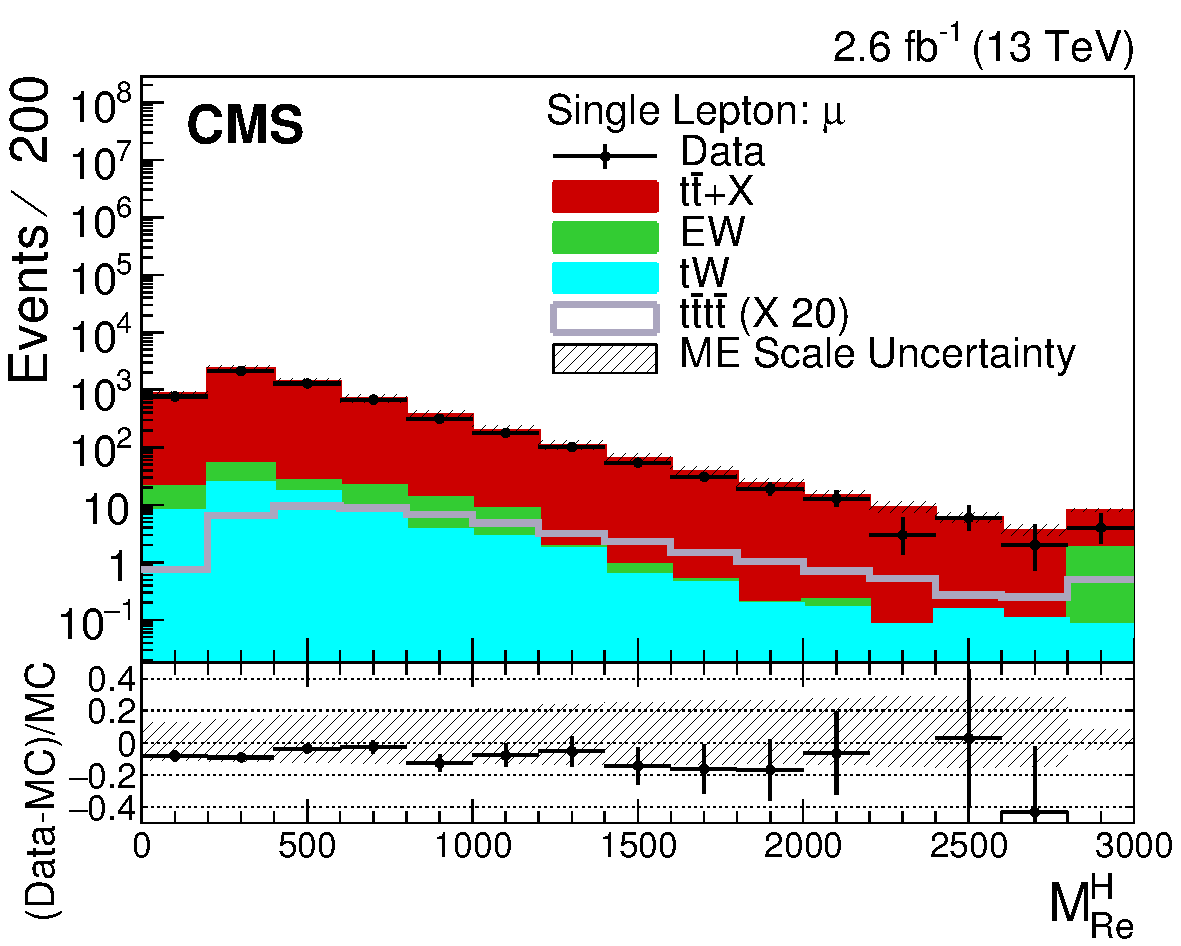
\includegraphics[width=0.44\textwidth]{images/Run2/SumJetMassX_StackLogY.pdf}
    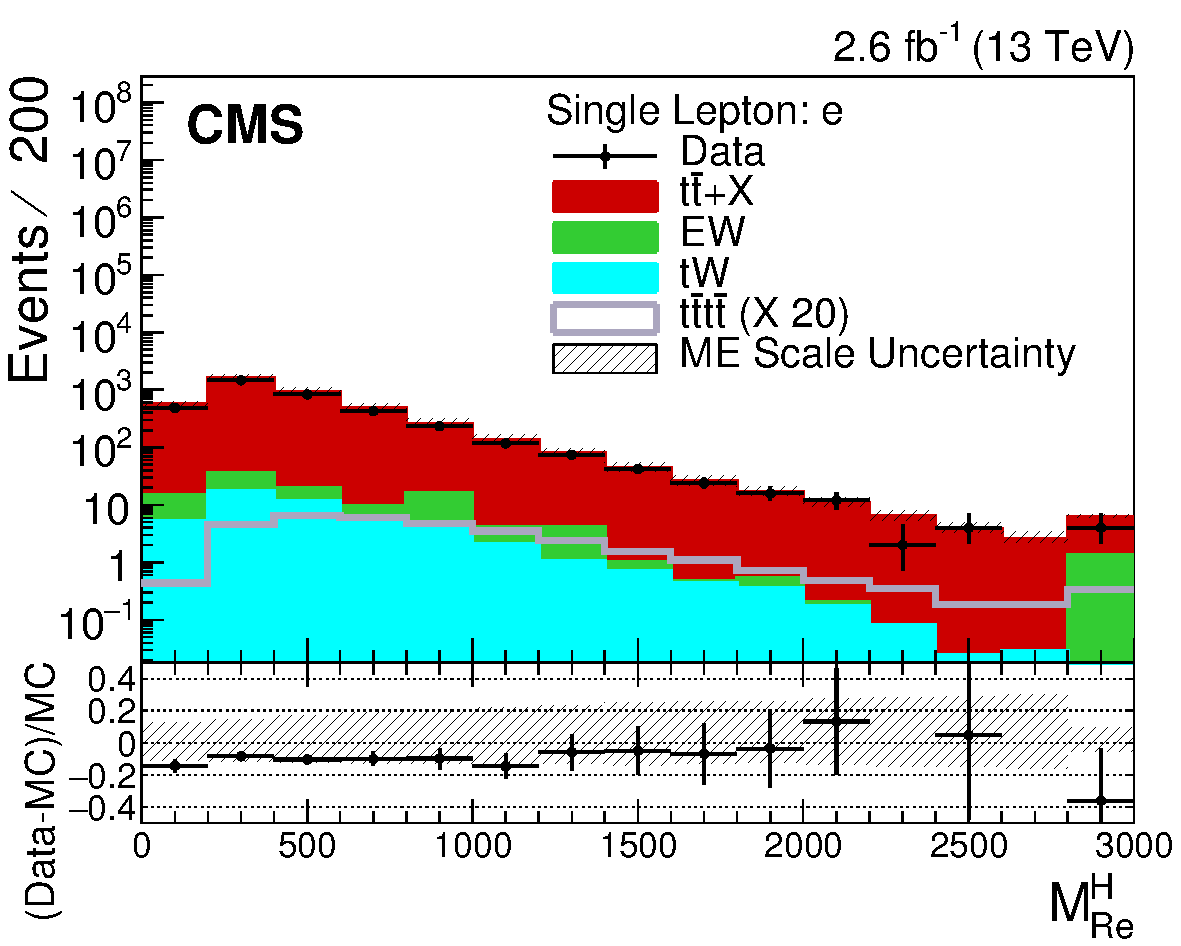
\includegraphics[width=0.44\textwidth]{images/Run2/SumJetMassX_StackLogY_e.pdf}
    \caption{ The \redhadmass distributions for data and simulation event in the $\mu$ + jets channel (left) and $e$ + jets channel (right) are plotted.}
    \label{fig:sumjetmassx13}
\end{figure}


\subsection{Event activity and b-jet content variables chosen for the event-level BDT}
The following variables were chosen for their discrimination power within the event-level BDT and are previously described in Section~\ref{sec:Strategy}. It should be noted that the third-highest CSV and fourth-highest CSV values can be used in the $\sqrt{s} = 13$~TeV analysis as the CSV distributions have been corrected by the modelling in Section~\ref{subsec:method2btag}.


\begin{multicols}{2}
\setlength{\columnseprule}{0pt} 

\begin{itemize}
\item \htb
\item \htrat
\item \njets
\item lepton \pt, \leadleppt
\item \njetsw
\item third-highest CSV
\item fourth-highest CSV
\end{itemize}

\end{multicols}

\subsection{Event-level BDT}
A \ttbar sample and a \tttt sample is provided to the TMVA package to train and test the performance of the event-level BDT using the AdaBoost boosting algorithm~\cite{FREUND1997119} was used. The \MADGRAPH\aMCATNLO \tttt sample was used with all negative weights set to one in the training. The gradient boosting algorithm~\cite{mason1999boosting} can be used with negative weights hence it was used to verify that the inclusion of negative weights (or not) had negligible impact on the final limit. Ultimately the AdaBoost algorithm produced a stronger limit on the \tttt cross section than the gradient boosting algorithm with the negative weights set to one. The jet modelling scale factor weight from Section~\ref{subsec:alphaS} is supplied to the BDT as it is important to correct the mismodelling of the most powerful variable input into the BDT.\\
The separation of the input variables, before any boost weights are applied, is shown in Fig.~\ref{fig:BDTInputVars} and the ranking of the variables in terms of variable importance are shown for the muon channel in Table~\ref{tab:BDTrankings}. The variables \njets, third-highest CSV and \htrat are the highest ranked variables and their discriminating power is evident in their initial separation power. The lowest ranked variable is \leadleppt, which is also seen in Fig.~\ref{fig:BDTInputVars} to have poor separation power initially. However it still enhances the discrimination power of the BDT to include the \leadleppt variable and it is preferable to have at least one leptonic variable in the list of input variables rather than all hadronic variables.

\begin{figure}[h!]
    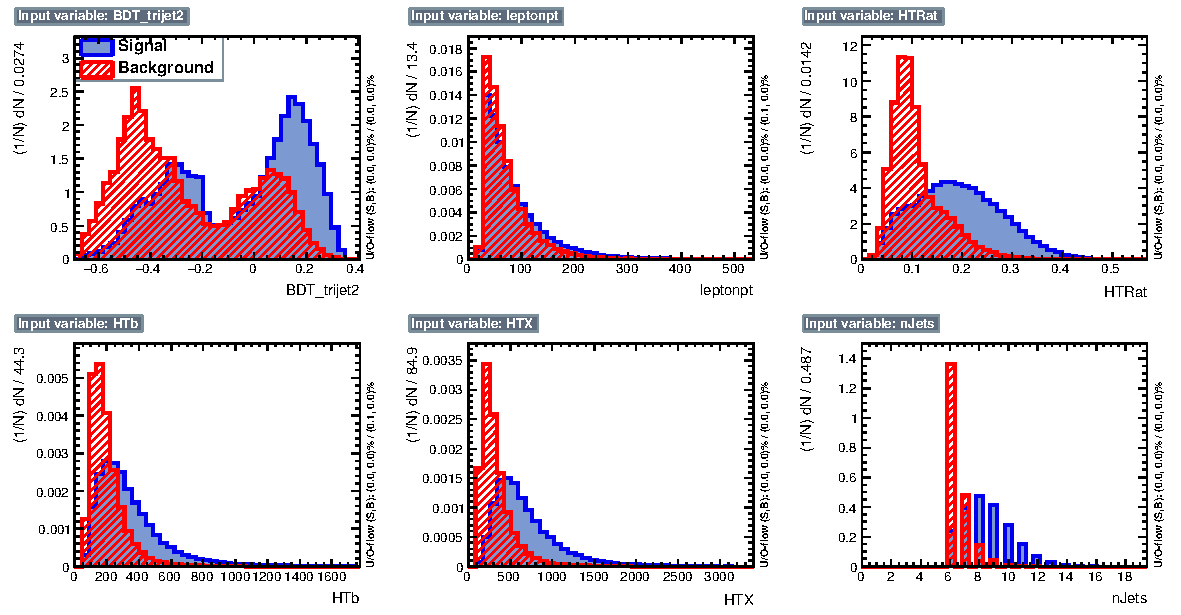
\includegraphics[width=\textwidth]{images/Run2/variables_id_c1_ELBDT13.pdf}\\
    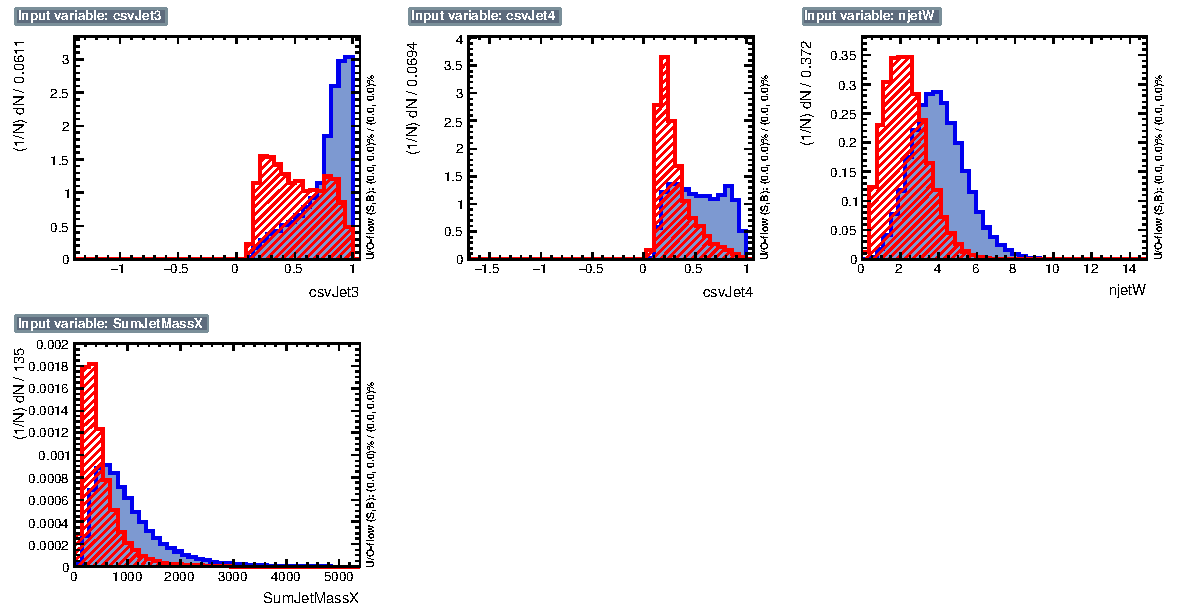
\includegraphics[width=\textwidth]{images/Run2/variables_id_c2_ELBDT13.pdf}
    \caption{Normalised distributions of the input variables in the muon channel taken from TMVA}
    \label{fig:BDTInputVars}
\end{figure}

\begin{table}[ht!]
\centering
\begin{tabular}{| l | l | l | p{5cm} |}
  \hline
Rank & Variable & Importance \\
 \hline
1 & \njets & 1.340e-01\\
2 & third-highest CSV &1.180e-01\\
3 & \htrat & 1.133e-01\\
4 & BDT$_{trijet2}$ & 1.091e-01 \\
5 & \njetsw &1.082e-01\\
6 & \redhadmass& 1.026e-01\\
7 & \HTX & 9.867e-02\\
8 & \htb & 8.650e-02 \\
9 & fourth-highest CSV & 7.630e-02\\
10 & \leadleppt & 5.334e-02  \\
\hline
\end{tabular}
 \caption{Ranking of variables in order of discrimination power within the BDT.}
  \label{tab:BDTrankings}
  \end{table}

The output discriminator value for the event level BDT is split into \njets categories of 6, 7, 8 and $\geq$9 jets and further to the \runone analysis in Chapter~\ref{c:Run1}, the distributions are also split into \nMtags categories of 2, 3 and $\geq$4 b-tags which further splits the distributions into regions which are more sensitive to the signal and regions which are better for constraining the background.
The output BDT plots are shown in \njets and \nMtags categories in Figs.~\ref{fig:BDT_Mu29Aug400trees_5MinNodeSize_20nCuts_3MaxDepth_5adaboostbeta_adaBoost_alphaSTune_noMinEvents62}~-~\ref{fig:BDT_Mu29Aug400trees_5MinNodeSize_20nCuts_3MaxDepth_5adaboostbeta_adaBoost_alphaSTune_noMinEvents94}. It can be seen that the signal becomes more separated from the background in the higher \njets and \nMtags categories as it moves towards higher BDT discriminator values. The lower \njets and \nMtags categories can help to constrain the \ttbar background. These categories act like control regions due to the very large background to signal ratio.

\begin{figure}[ht!]
    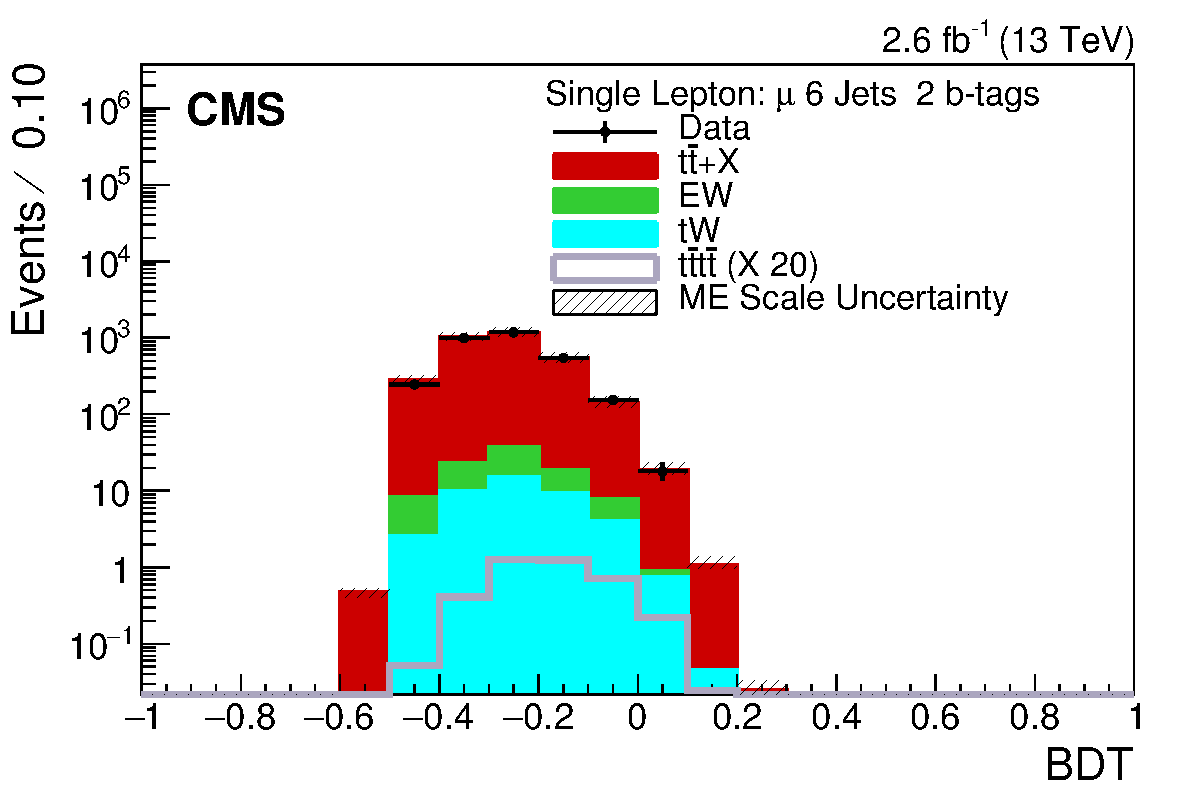
\includegraphics[width=0.48\textwidth]{images/Run2/BDT_Mu29Aug400trees_5MinNodeSize_20nCuts_3MaxDepth_5adaboostbeta_adaBoost_alphaSTune_noMinEvents6nJets2nMtags_StackLogY.pdf}
    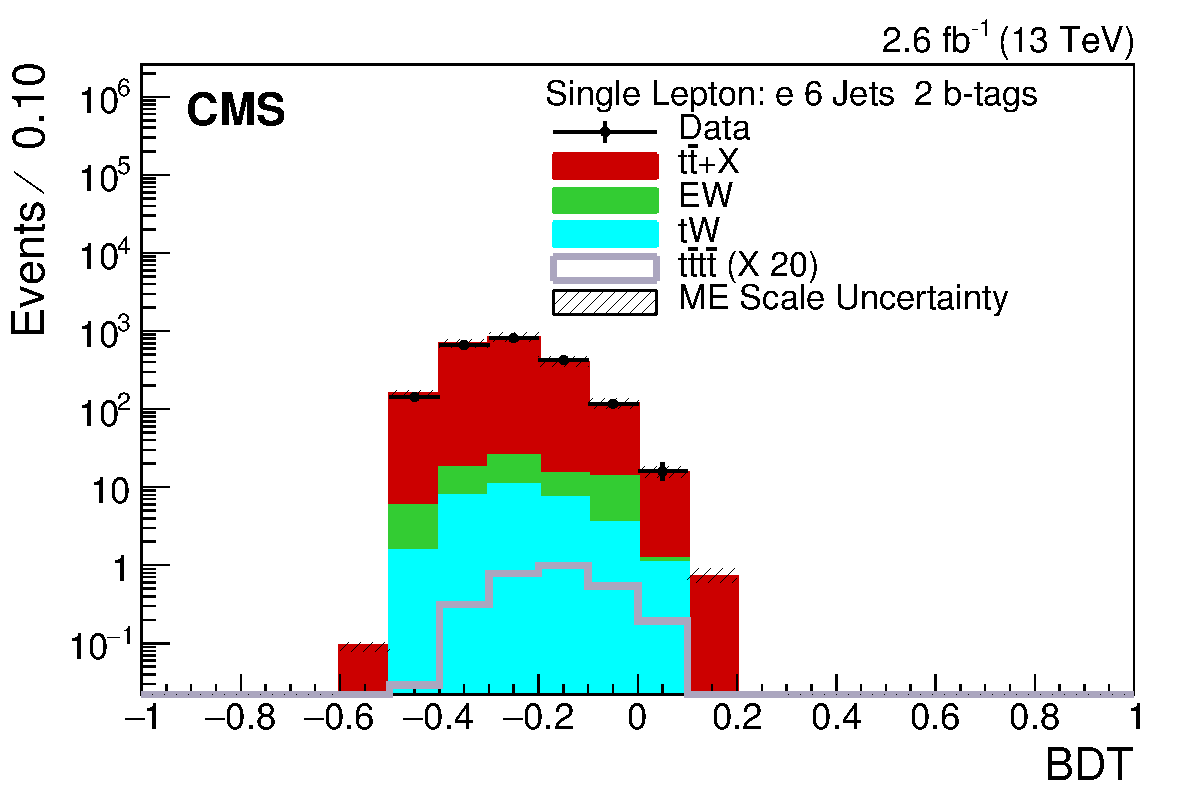
\includegraphics[width=0.48\textwidth]{images/Run2/BDT_El29Aug400trees_5MinNodeSize_20nCuts_3MaxDepth_5adaboostbeta_adaBoost_alphaSTune_noMinEvents6nJets2nMtags_StackLogY.pdf} 
    \caption{The BDT output distributions for AdaBoost for data and simulation in the $\mu$ + jets channel (left) and e + jets channel (left) are shown for the 6 \njets and 2\nMtags category.}
    \label{fig:BDT_Mu29Aug400trees_5MinNodeSize_20nCuts_3MaxDepth_5adaboostbeta_adaBoost_alphaSTune_noMinEvents62}
\end{figure}

\begin{figure}[ht!]
    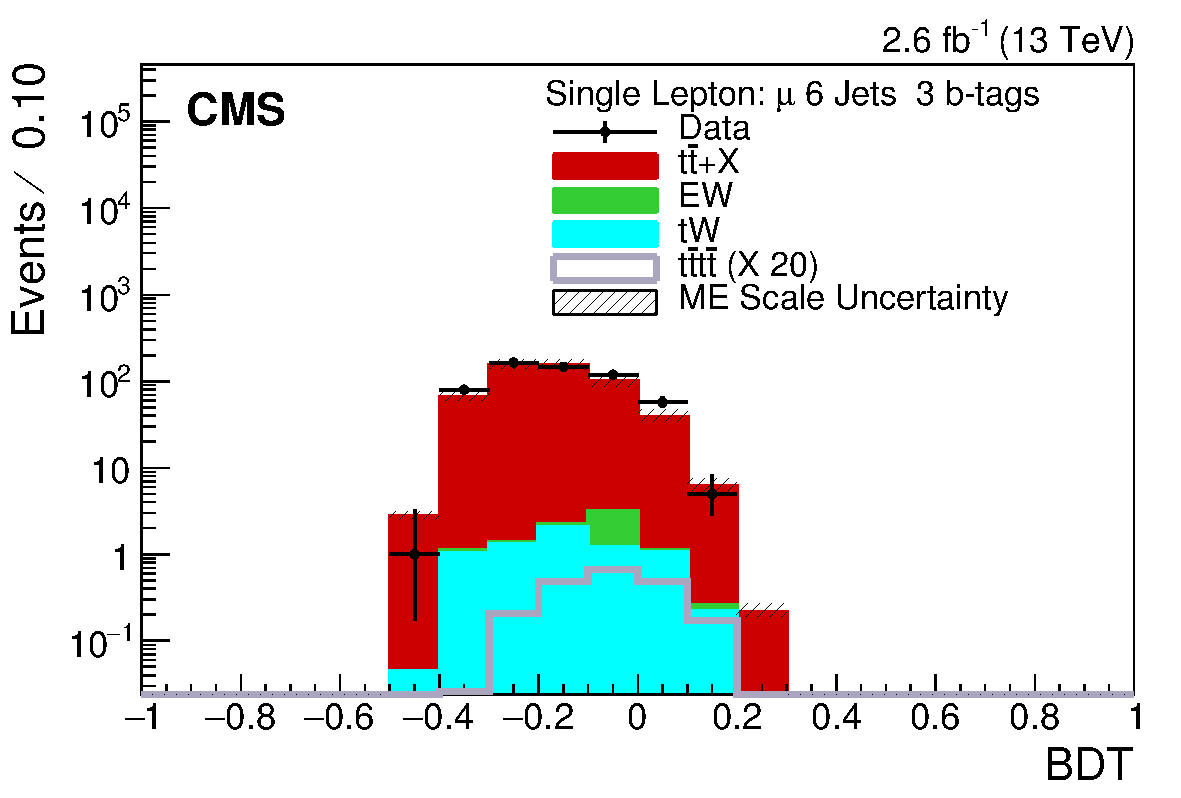
\includegraphics[width=0.48\textwidth]{images/Run2/BDT_Mu29Aug400trees_5MinNodeSize_20nCuts_3MaxDepth_5adaboostbeta_adaBoost_alphaSTune_noMinEvents6nJets3nMtags_StackLogY.pdf}
    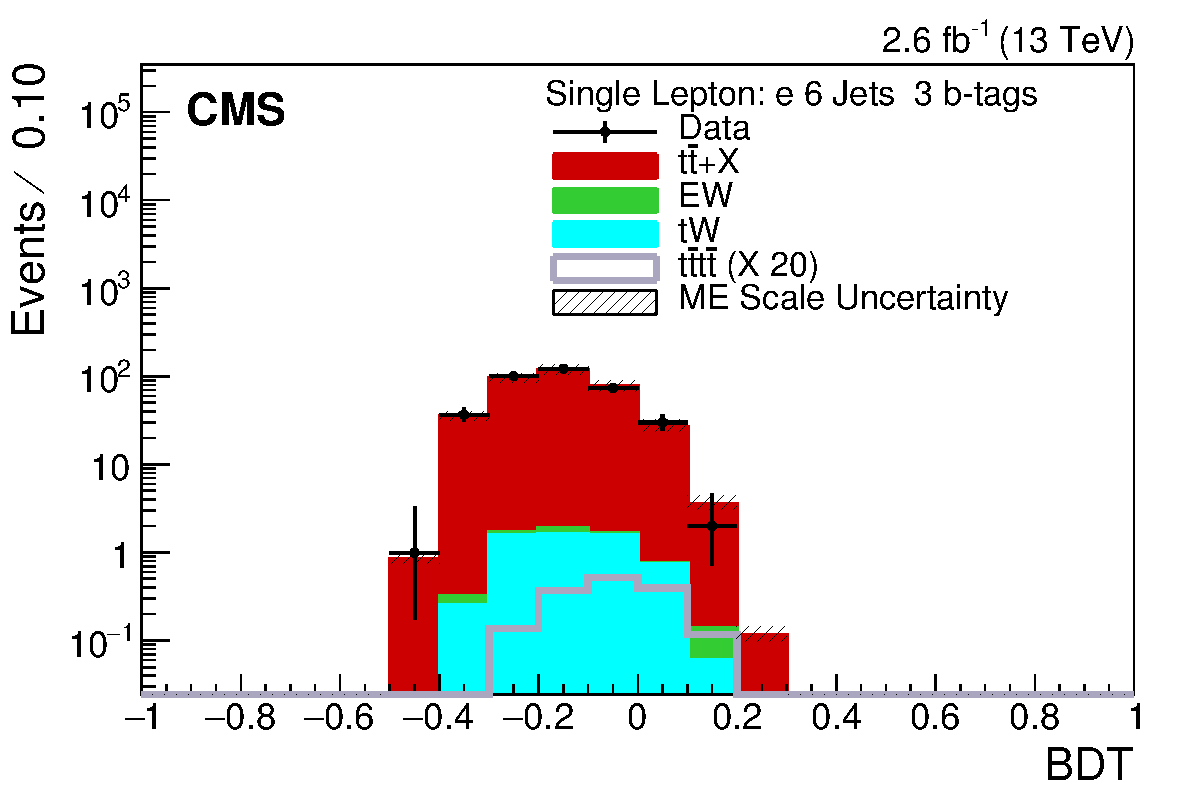
\includegraphics[width=0.48\textwidth]{images/Run2/BDT_El29Aug400trees_5MinNodeSize_20nCuts_3MaxDepth_5adaboostbeta_adaBoost_alphaSTune_noMinEvents6nJets3nMtags_StackLogY.pdf} 
    \caption{The BDT output distributions for AdaBoost for data and simulation in the $\mu$ + jets channel (left) and e + jets channel (left) are shown for the 6 \njets and 3\nMtags category.}
    \label{fig:BDT_Mu29Aug400trees_5MinNodeSize_20nCuts_3MaxDepth_5adaboostbeta_adaBoost_alphaSTune_noMinEvents63}
\end{figure}

\begin{figure}[ht!]
    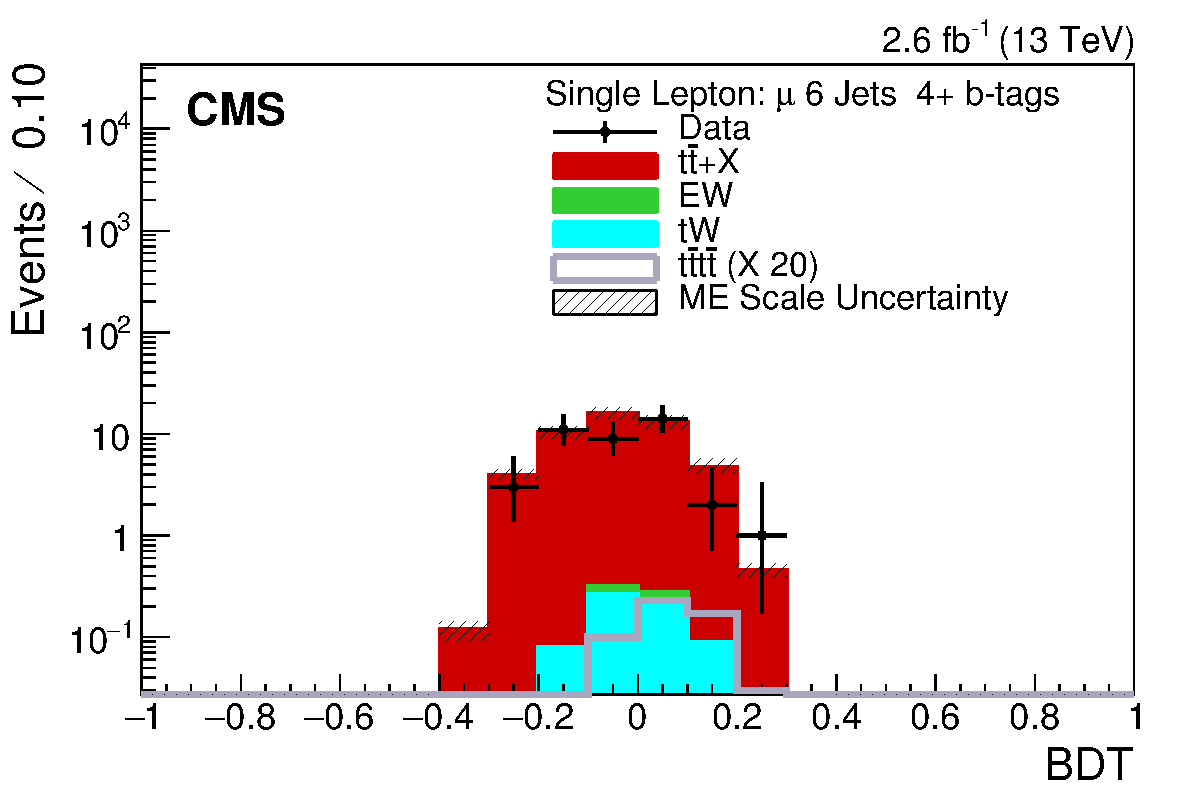
\includegraphics[width=0.48\textwidth]{images/Run2/BDT_Mu29Aug400trees_5MinNodeSize_20nCuts_3MaxDepth_5adaboostbeta_adaBoost_alphaSTune_noMinEvents6nJets4nMtags_StackLogY.pdf}
    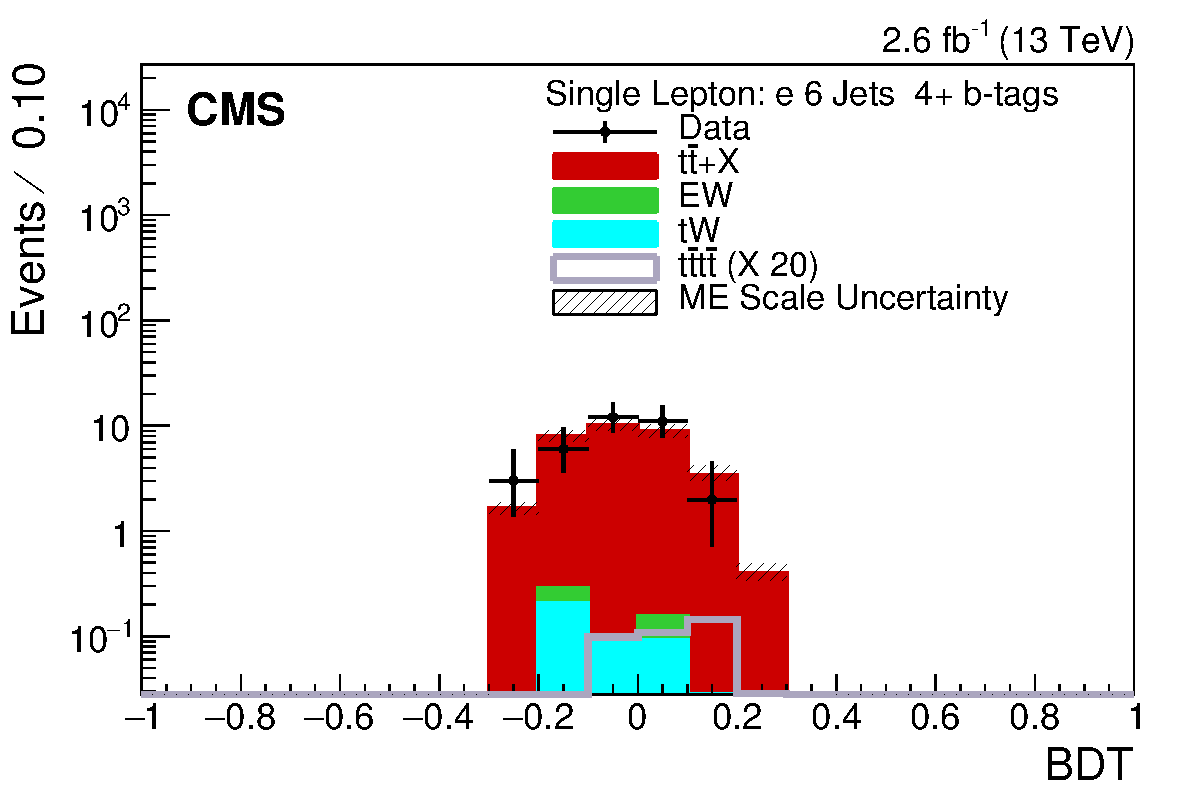
\includegraphics[width=0.48\textwidth]{images/Run2/BDT_El29Aug400trees_5MinNodeSize_20nCuts_3MaxDepth_5adaboostbeta_adaBoost_alphaSTune_noMinEvents6nJets4nMtags_StackLogY.pdf}
    \caption{The BDT output distributions for AdaBoost for data and simulation in the $\mu$ + jets channel (left) and e + jets channel (right) are shown for the 6 \njets and $\geq4$ \nMtags category.}
    \label{fig:BDT_Mu29Aug400trees_5MinNodeSize_20nCuts_3MaxDepth_5adaboostbeta_adaBoost_alphaSTune_noMinEvents64}
\end{figure}

\begin{figure}[ht!]
    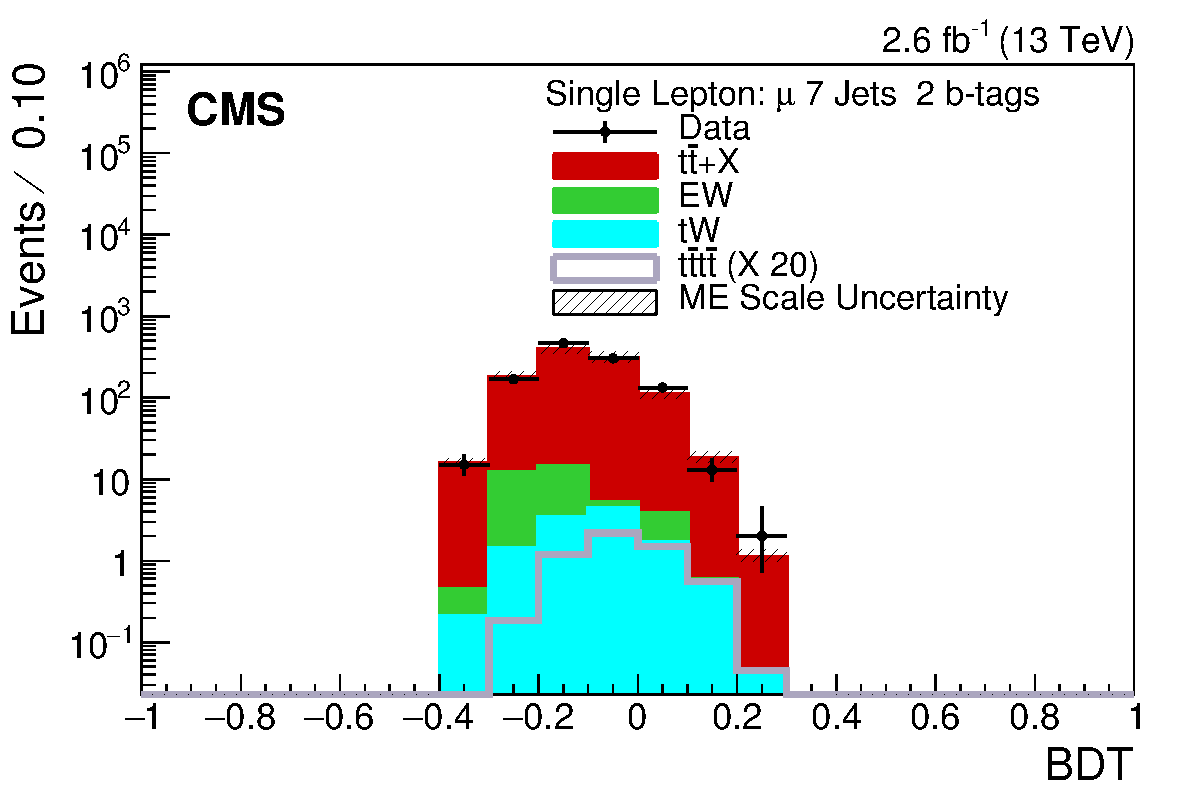
\includegraphics[width=0.48\textwidth]{images/Run2/BDT_Mu29Aug400trees_5MinNodeSize_20nCuts_3MaxDepth_5adaboostbeta_adaBoost_alphaSTune_noMinEvents7nJets2nMtags_StackLogY.pdf}
    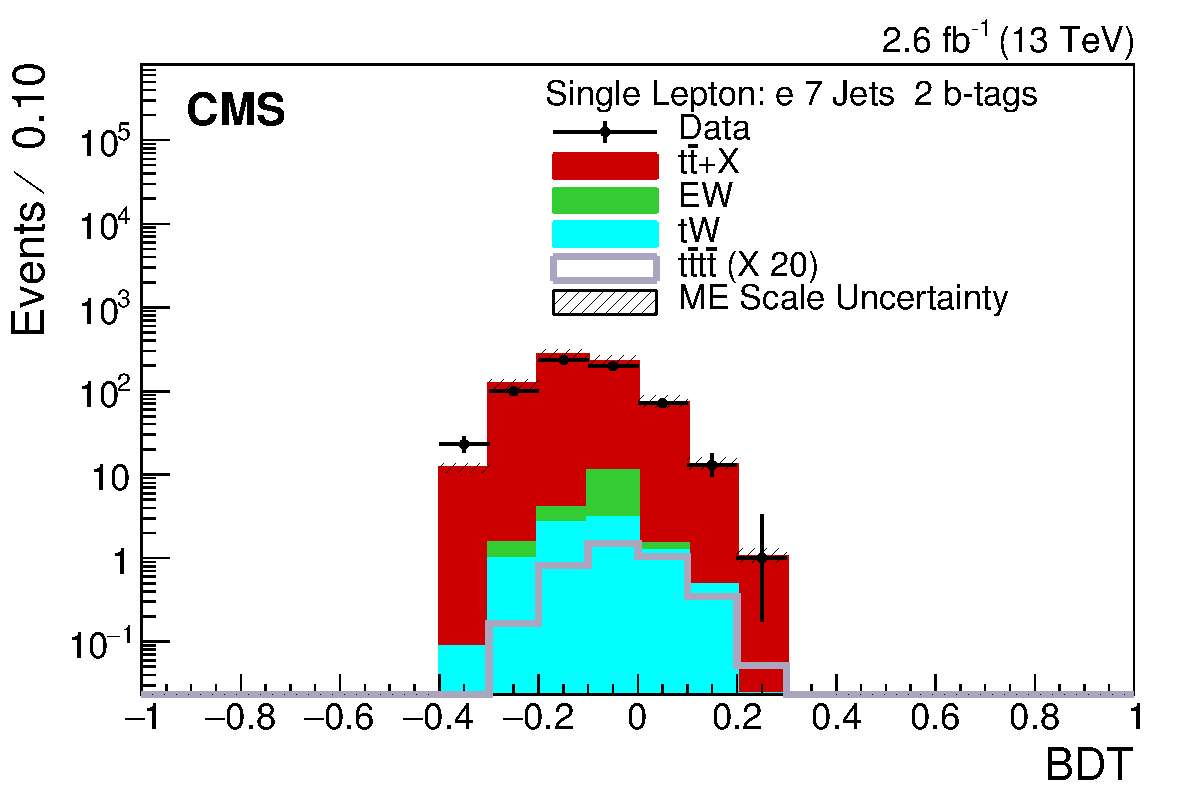
\includegraphics[width=0.48\textwidth]{images/Run2/BDT_El29Aug400trees_5MinNodeSize_20nCuts_3MaxDepth_5adaboostbeta_adaBoost_alphaSTune_noMinEvents7nJets2nMtags_StackLogY.pdf} 
    \caption{The BDT output distributions for AdaBoost for data and simulation in the $\mu$ + jets channel (left) and e + jets channel (left) are shown for the 7 \njets and 2 \nMtags category.}
    \label{fig:BDT_Mu29Aug400trees_5MinNodeSize_20nCuts_3MaxDepth_5adaboostbeta_adaBoost_alphaSTune_noMinEvents72}
 \end{figure}

\begin{figure}[ht!]
    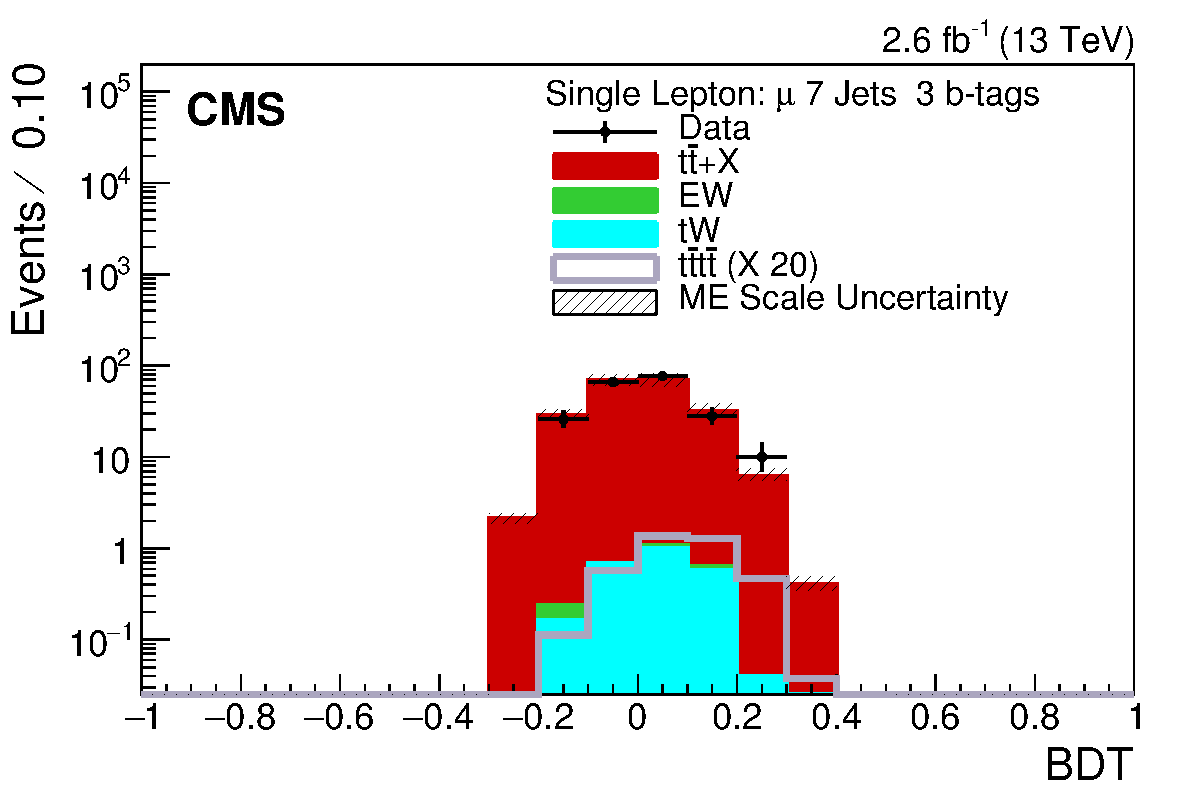
\includegraphics[width=0.48\textwidth]{images/Run2/BDT_Mu29Aug400trees_5MinNodeSize_20nCuts_3MaxDepth_5adaboostbeta_adaBoost_alphaSTune_noMinEvents7nJets3nMtags_StackLogY.pdf}
    \includegraphics[width=0.48\textwidth]{images/Run2/BDT_El29Aug400trees_5MinNodeSize_20nCuts_3MaxDepth_5adaboostbeta_adaBoost_alphaSTune_noMinEvents7nJets3nMtags_StackLogY.pdf}
    \caption{The BDT output distributions for AdaBoost for data and simulation in the $\mu$ + jets channel (left) and e + jets channel (left) are shown for the 7 \njets and 3 \nMtags category.}
    \label{fig:BDT_Mu29Aug400trees_5MinNodeSize_20nCuts_3MaxDepth_5adaboostbeta_adaBoost_alphaSTune_noMinEvents73}
 \end{figure}

\begin{figure}[ht!]
    \includegraphics[width=0.48\textwidth]{images/Run2/BDT_Mu29Aug400trees_5MinNodeSize_20nCuts_3MaxDepth_5adaboostbeta_adaBoost_alphaSTune_noMinEvents7nJets4nMtags_StackLogY.pdf}
    \includegraphics[width=0.48\textwidth]{images/Run2/BDT_El29Aug400trees_5MinNodeSize_20nCuts_3MaxDepth_5adaboostbeta_adaBoost_alphaSTune_noMinEvents7nJets4nMtags_StackLogY.pdf}
    \caption{The BDT output distributions for AdaBoost for data and simulation in the $\mu$ + jets channel (left) and e + jets channel (right) are shown for the 7 \njets and $\geq4$ \nMtags category.}
    \label{fig:BDT_Mu29Aug400trees_5MinNodeSize_20nCuts_3MaxDepth_5adaboostbeta_adaBoost_alphaSTune_noMinEvents74}
\end{figure}

\begin{figure}[ht!]
    \includegraphics[width=0.48\textwidth]{images/Run2/BDT_Mu29Aug400trees_5MinNodeSize_20nCuts_3MaxDepth_5adaboostbeta_adaBoost_alphaSTune_noMinEvents8nJets2nMtags_StackLogY.pdf}
    \includegraphics[width=0.48\textwidth]{images/Run2/BDT_El29Aug400trees_5MinNodeSize_20nCuts_3MaxDepth_5adaboostbeta_adaBoost_alphaSTune_noMinEvents8nJets2nMtags_StackLogY.pdf} 
    \caption{The BDT output distributions for AdaBoost for data and simulation in the $\mu$ + jets channel (left) and $e$ + jets channel (left) are shown for the 8 \njets and 2 \nMtags category.}
    \label{fig:BDT_Mu29Aug400trees_5MinNodeSize_20nCuts_3MaxDepth_5adaboostbeta_adaBoost_alphaSTune_noMinEvents82}
\end{figure}

\begin{figure}[ht!]
    \includegraphics[width=0.48\textwidth]{images/Run2/BDT_Mu29Aug400trees_5MinNodeSize_20nCuts_3MaxDepth_5adaboostbeta_adaBoost_alphaSTune_noMinEvents8nJets3nMtags_StackLogY.pdf}
    \includegraphics[width=0.48\textwidth]{images/Run2/BDT_El29Aug400trees_5MinNodeSize_20nCuts_3MaxDepth_5adaboostbeta_adaBoost_alphaSTune_noMinEvents8nJets3nMtags_StackLogY.pdf} 
    \caption{The BDT output distributions for AdaBoost for data and simulation in the $\mu$ + jets channel (left) and $e$ + jets channel (left) are shown for the 8 \njets category and 3 \nMtags category.}
    \label{fig:BDT_Mu29Aug400trees_5MinNodeSize_20nCuts_3MaxDepth_5adaboostbeta_adaBoost_alphaSTune_noMinEvents83}
\end{figure}

\begin{figure}[ht!]
    \includegraphics[width=0.48\textwidth]{images/Run2/BDT_Mu29Aug400trees_5MinNodeSize_20nCuts_3MaxDepth_5adaboostbeta_adaBoost_alphaSTune_noMinEvents8nJets4nMtags_StackLogY.pdf}
    \includegraphics[width=0.48\textwidth]{images/Run2/BDT_El29Aug400trees_5MinNodeSize_20nCuts_3MaxDepth_5adaboostbeta_adaBoost_alphaSTune_noMinEvents8nJets4nMtags_StackLogY.pdf}
    \caption{The BDT output distributions for AdaBoost for data and simulation in the $\mu$ + jets channel (left) and $e$ + jets channel (right) are shown for the 8 \njets and $\geq4$ \nMtags category.}
    \label{fig:BDT_Mu29Aug400trees_5MinNodeSize_20nCuts_3MaxDepth_5adaboostbeta_adaBoost_alphaSTune_noMinEvents84}
\end{figure}

\newpage

\begin{figure}[ht!]
    \includegraphics[width=0.48\textwidth]{images/Run2/BDT_Mu29Aug400trees_5MinNodeSize_20nCuts_3MaxDepth_5adaboostbeta_adaBoost_alphaSTune_noMinEvents9nJets2nMtags_StackLogY.pdf}
    \includegraphics[width=0.48\textwidth]{images/Run2/BDT_El29Aug400trees_5MinNodeSize_20nCuts_3MaxDepth_5adaboostbeta_adaBoost_alphaSTune_noMinEvents9nJets2nMtags_StackLogY.pdf} 
    \caption{The BDT output distributions for AdaBoost for data and simulation in the $\mu$ + jets channel (left) and $e$ + jets channel (left) are shown for the $\geq9$ \njets  and 2 \nMtags category.}
    \label{fig:BDT_Mu29Aug400trees_5MinNodeSize_20nCuts_3MaxDepth_5adaboostbeta_adaBoost_alphaSTune_noMinEvents92}
\end{figure}

\begin{figure}[ht!]
    \includegraphics[width=0.48\textwidth]{images/Run2/BDT_Mu29Aug400trees_5MinNodeSize_20nCuts_3MaxDepth_5adaboostbeta_adaBoost_alphaSTune_noMinEvents9nJets3nMtags_StackLogY.pdf}
    \includegraphics[width=0.48\textwidth]{images/Run2/BDT_El29Aug400trees_5MinNodeSize_20nCuts_3MaxDepth_5adaboostbeta_adaBoost_alphaSTune_noMinEvents9nJets3nMtags_StackLogY.pdf}
    \caption{The BDT output distributions for AdaBoost for data and simulation in the $\mu$ + jets channel (left) and $e$ + jets channel (left) are shown for the $\geq9$ \njets  and 3 \nMtags category.}
    \label{fig:BDT_Mu29Aug400trees_5MinNodeSize_20nCuts_3MaxDepth_5adaboostbeta_adaBoost_alphaSTune_noMinEvents93}
\end{figure}

\begin{figure}[ht!]
    \includegraphics[width=0.48\textwidth]{images/Run2/BDT_Mu29Aug400trees_5MinNodeSize_20nCuts_3MaxDepth_5adaboostbeta_adaBoost_alphaSTune_noMinEvents9nJets4nMtags_StackLogY.pdf}
    \includegraphics[width=0.48\textwidth]{images/Run2/BDT_El29Aug400trees_5MinNodeSize_20nCuts_3MaxDepth_5adaboostbeta_adaBoost_alphaSTune_noMinEvents9nJets4nMtags_StackLogY.pdf}    
    \caption{The BDT output distributions for AdaBoost for data and simulation in the $\mu$ + jets channel (left) and $e$ + jets channel (right) are shown for the $\geq9$ \njets and $\geq4$ \nMtags category.}
    \label{fig:BDT_Mu29Aug400trees_5MinNodeSize_20nCuts_3MaxDepth_5adaboostbeta_adaBoost_alphaSTune_noMinEvents94}
\end{figure}

The BDT was seen to be very stable with respect to changes in the number of trees used and to the minimum number of events required at a node for further splitting to occur. The impact on the final expected limit was negligible when changing these BDT hyperparameters. Training was also performed in jet categories of 6-7 jets and $\geq$8 jets separately to study whether a separate training in the $\geq8$ jets category would improve the power of the BDT to separate \ttbar and \tttt events in a signal-rich region. However the expected limit derived from this alternative training was not enhanced with respect to the inclusive training in all jet categories. The most significant improvement in the expected limit came from optimising the \njets and \nMtags categories. Further categorisation into higher \njets and \nMtags categories improves the expected limit however these categories become very statistically limited with 2.6~\fbinv of data.

\section{Systematic uncertainties}
\label{sec:uncertainties13}
All systematic uncertainties are described in Section~\ref{sec:uncertainties} and some further details about them are given below.

\begin{itemize}
\item \textbf{Luminosity}\\
The CMS Luminosity Group gave a recommendation of 2.7$\%$ uncertainty on the luminosity~\cite{CMS-PAS-LUM-15-001} which is applied to all backgrounds.
\item \textbf{Monte Carlo cross sections}\\
The uncertainty on the main background of \ttbar is ${}^{+2.5\%}_{-3.4\%}$ renormalisation and factorisation scale and ${}^{+6.2\%}_{-6.4\%} \left( \textrm{PDF} \right)$~\cite{PhysRevLett.110.252004}. The MC cross section uncertainties for the other background processes are modelled by assigning a $4\%$ uncertainty and a $10\%$ uncertainty is assigned to the signal process.
\item \textbf{Lepton SF}\\
The lepton SF is applied to all backgrounds. The uncertainty on these Sfs is 1.3$\%$ in muon channel and 3.6$\%$ in electron channel
\item \textbf{Matrix Element Factorisation and renormalisation scales}\\
Weights are available in the \ttbar and \tttt samples which correspond to the factorisation and renormalisation scale $\left(\mu_{f},~\mu_{s}\right)$ being individually varied through 1/2u, u and 2u, where u represents the central value. This gives nine weights however the extreme unphysical values of (1/2u, 1/2u) and (2u, 2u) are not included. Applying these weights individually gives six alternative event-level BDT histograms to the central histogram, which uses (u,u). 
\item \textbf{Parton Shower Factorisation and renormalisation scales}\\
The effect of the parton showering (PS) scale in the \PYTHIA~8 generator is evaluated by using alternative \ttbar samples with the PS scale (u$_{PS}$) varied by 2u$_{PS}$, 1/2u$_{PS}$. This shift in the PS scale is equivalent to modifying the value of $\alpha_{S}$ hence the alternative parton shower histogram shapes have been inflated by a factor of 1.5 relative to the nominal template to take into account the uncertainty on the jet multiplicity modelling.
\item \textbf{\ttbar generator}\\
The \POWHEG generator was used to produce the nominal \ttbar sample for this analysis. This can be compared to running the analysis with the \MLM and \MADGRAPH\aMCATNLO~FxFx \ttbar samples. A symmetric envelope could be formed around the nominal by symmetrising the difference in event counts in each bin between the alternative and nominal samples. The \MLM sample was found to produce the most conservative uncertainty for this effect and so it was used to produce the symmetric up and down histograms.
\item \textbf{JES}\\
The JES uncertainty is derived by varying the JES by $\pm1\sigma$ for the \ttbar and \tttt samples.
\item \textbf{JER}\\
The JER uncertainty is derived by varying the smearing by $\pm1\sigma$ for the \ttbar and \tttt samples.
\item \textbf{b tagging}\\
As detailed in Section~\ref{sec:Calibrations13}, the difference between b-tagging efficiency in data and simulation is accounted for by the application of scale factors to simulated events via an event weighting procedure. This is the event weighting procedure was developed in Ref.~\cite{CMS-PAS-HIG-16-004}, details of which are documented here~\cite{CMS-NOTE-2013-130}. Given the significant uncertainty on these scale factors and that the CSV distributions are input variables to the BDT algorithm, a significant systematic effect is expected. Light flavour, `lf', and linear statistical and quadratic statistical fluctuations, `hfstats1' and `hfstats2', are applied to heavy flavour jets.  Heavy flavour, `hf', and linear statistical and quadratic statistical fluctuations, `lfstats1' and `lfstats2', are applied to light flavour jets. Linear and quadratic uncertainties, `cferr1' and `cferr2', are applied to charm flavour jets. A b-tagging JES systematic is applied to light and heavy flavour jets when the standard jet energy scale systematics are applied and hence it is incorporated into the alternative JES systematic shapes. The b-tagging systematic is studied for the \ttbar and \tttt samples.
\item \textbf{Pile up}\\
The PU systematic uncertainty is found by varying the MinBias cross section by $\pm5\%$ and is applied to the \ttbar and \tttt samples.
\item \textbf{\heavyflavourone / \heavyflavourtwo modelling}
The uncertainty on the measurement of \heavyflavourone / \heavyflavourtwo by CMS~\cite{Khachatryan2015132} is $\pm 0.3 \left( \textrm{stat.} \right) \pm 0.6 \left(\textrm{sys.} \right)$. Alternative event weights are derived for \heavyflavourone / \heavyflavourtwo which are used to provide the alternative systematic up and down histograms.
\end{itemize}
\section{Template fit and upper limit}
\label{sec:limit13}
As no excess of events over the background expectation consistent with SM $\tttt$ production was observed, upper limits on $\sigma_{\tttt}^{SM}$ are calculated. 
The limit setting proceeds by simultaneously fitting the BDT output distributions of signal and backgrounds to the BDT distribution of data in both the $\mu$ + jets and $e$ + jets channels in all 12 \njets and \nMtags categories. The Higgs Combined Tool is used to perform the fit, assigning lognormal uncertainties to normalisation systematic uncertainties and the vertical morphing technique described in Section~\ref{sec:limitFit} for the shape systematic uncertainties. The fit produces a fitted shape and normalisation and best-fit values for all nuisance parameters and the parameter of interest. 
To avoid prohibitively large computing times, the approximate \emph{asymptotic} approach is used to calculate the \CLS limits, which can be found in Table~\ref{tab:limits} in units of $\sigma_{SM}$. 

\begin{table}[ht!]
\centering
\begin{tabular}{| l | c | c | c | c | c |}
  \hline
Channel  & Categorized & Uncertainty & Observed\\
 \hline
$\mu$  &$20.6$ & $+12.9 -7.2$ & $20.8$ \\
 \hline
e  &  $26.4$ & $+16.6 -9.3$ & $33.5$ \\
 \hline
 Combined  &  $16.0$ & $+9.8 -5.5$ & $16.8$ \\
 \hline
\end{tabular}
 \caption{Extracted expected limits for \njets and \nMtags categorized templates in multiples of $\sigma_{SM}$.}
  \label{tab:limits}
  \end{table}

The combined expected limit is $147.2^{+90}_{-51}$~fb and the observed limit is 154.6~fb for the single lepton + jets channel.

\section{Systematics studies and tests on analysis}

% \subsection{Ranking of variables in BDT}

% \begin{table}[ht!]
% \centering
% \begin{tabular}{| l | l | l | p{5cm} |}
%   \hline
% Rank & Variable & Importance \\
%  \hline
% 1 & \njets & 1.340e-01\\
% 2 & third highest CSV &1.180e-01\\
% 3 & \htrat & 1.133e-01\\
% 4 & BDT$_{trijet2}$ & 1.091e-01 \\
% 5 & \njetsw &1.082e-01\\
% 6 & \redhadmass& 1.026e-01\\
% 7 & HTX & 9.867e-02\\
% 8 & \htb & 8.650e-02 \\
% 9 & fourth highest CSV & 7.630e-02\\
% 10 & leadleppt & 5.334e-02  \\

% \hline
% \end{tabular}
%  \caption{Ranking of variables in order of discrimination power within the BDT.}
%   \label{tab:BDTrankings}
%   \end{table}

\subsection{Correlation Matrices}

% The correlation matrices for signal and background are shown in Fig.~\ref{fig:corrMat}. The largest correlation exists between \njetsw and \redhadmass. This is not surprising as \njetsw takes into account the weight of jets above a pt threshold and \redhadmass is the invariant mass of the reduced event. Many high pt jets in an event will correspond to a larger value of \redhadmass. 
% Correlated variables are handled well within a BDT and that was one of the reasons for the choice of this type of multivariate algorithm. The correlation matrices were used at an earlier stage in the analysis to assess what variables were very highly correlated and could be removed from the input BDT variables as they would serve little use within the BDT.

Figure~\ref{fig:corrMat} shows the correlation matrices for the input BDT variables for the background \ttbar (left) and signal \tttt (right). It can be seen that the most highly correlated variables are \njetsw and \redhadmass. This correlation arises from the fact that the \njetsw variable weights events by the \pt of jets and more additional higher-\pt jets will lead to a larger value of \redhadmass.\\
BDTs are effective at handling correlated variables and this was one reason for the chosen of using this multivariate algorithm.

Correlation matrices were used when choosing which variables to include in the final set which was used to train the BDT for this analysis. Highly correlated variables were removed as they are largely superfluous.

\begin{figure}[ht!]
    \includegraphics[width=0.48\textwidth]{images/Run2/CorrelationMatrixB.pdf}
    \includegraphics[width=0.48\textwidth]{images/Run2/CorrelationMatrixS.pdf}
    \caption{The correlation matrices for background (left) and signal (right).}
    \label{fig:corrMat}
\end{figure}

The correlation matrix for the fit nuisance parameters in the background only scenario can be see in Fig.~\ref{fig:FitCorr}. There is some correlation between the various b-tagging scale factors and also a correlation between the heavy flavour \heavyflavourone / \heavyflavourtwo modelling and the \ttbar ME scale, where the \heavyflavourone / \heavyflavourtwo is expected to be related to the choice is ME scale.

\begin{figure}[ht!]
    \includegraphics[width=0.9\textwidth]{images/Run2/FitCorr.pdf}
    \caption{The correlation matrices for background only for the fit parameters.}
    \label{fig:FitCorr}
\end{figure}

\subsection{Overtraining tests}

Figure~\ref{fig:ROC} shows the BDT distribution from training and testing (left) and the associated ROC curve for this training. The training sample is shown as a filled histogram and the testing sample is shown as overlaid data points for the signal \tttt (blue) and background \ttbar for red. It can be seen that there is good agreement between the training and testing samples with Kolmogorov-Smirnov values of 0.159 for background and 0.998 for signal. This suggest that the BDT has not been overtrained.

\begin{figure}
    \includegraphics[width=0.48\textwidth]{images/Run2/overtrain_BDT.pdf}
    \includegraphics[width=0.48\textwidth]{images/Run2/rejBvsS.pdf}
    \caption{The over-training test for the BDT (left) and the rejection of background \ttbar (red) vs signal \tttt (blue) (right).}
    \label{fig:ROC}
\end{figure}

\subsection{Nuisance parameters}

Figure~\ref{fig:datanuis} shows the variation of the post-fit nuisance parameters, $\theta$, with respect to their pre-fit values. As all of the parameters have not shifted outside of the pre-fit uncertainty, the number of uncertainties and their modelling is deduced to be appropriate for modelling the data. It can be seen that both the \ttbar ME scale uncertainty and the PS scale, denoted \emph{ttMEScale} and \emph{scaleH} respectively on the plot, have much smaller post-fit uncertainties with respect to their pre-fit uncertainties which suggests that they were over conservative.

\begin{figure}[h!]
\begin{center}
\subfloat{
\includegraphics[width=0.92\textwidth]{images/Run2/Nuisances.pdf}}
\hspace{0.2cm}
\end{center}
\caption{Post-fit nuisance parameters for data.}
\label{fig:datanuis}
\end{figure} 

\subsection{Studies of impact of systematic uncertainties}

The impact of each systematic uncertainty on the expected and observed limit is shown in Table~\ref{tab:sysRemoved} but removing each systematic from the fit.

\begin{table}[ht]
\centering
\caption{Limits on \tttt production which each systematic removed in turn}
\label{tab:sysRemoved}
\begin{tabular}{|l|l|l|}
\hline
Systematic uncertainty removed & Expected limit ($\times$\sigmattttsm) & Observed limit ($\times$\sigmattttsm) \\ \hline
None                           & 16.0000                             & 16.8340                             \\ \hline
\ttbar ME scale                & 16.0625                             & 16.4804                             \\ \hline
\tttt ME scale                 & 14.4375                             & 15.3639                             \\ \hline
JER                            & 15.9375                             & 16.9774                             \\ \hline
JES                            & 15.3125                             & 17.1332                             \\ \hline
PS scale                       & 15.0625                             & 15.7623                             \\ \hline
PU                             & 16.0625                             & 16.8574                             \\ \hline
Generator uncertainty          & 15.9531                             & 16.6530                             \\ \hline
\ttbar heavy flav              & 15.5625                             & 16.7846                             \\ \hline
Luminosity                     & 16.0625                             & 16.7553                             \\ \hline
Lepton SF Mu                   & 16.0625                             & 16.7646                             \\ \hline
Lepton SF El                   & 15.9062                             & 16.1287                             \\ \hline
\ttbar norm                    & 16.0000                             & 16.7771                             \\ \hline
\tttt norm                     & 15.9062                             & 16.7785                             \\ \hline
EW norm                        & 16.0000                             & 16.8358                             \\ \hline
Single top norm                & 16.0000                             & 16.8370                             \\ \hline
b-tag light SF                 & 12.5625                             & 15.8688                             \\ \hline
btagWeightCSVCFErr1            & 16.0625                             & 16.1875                             \\ \hline
btagWeightCSVCFErr2            & 16.0625                             & 16.8263                             \\ \hline
btagWeightCSVHF                & 15.5625                             & 15.5625                             \\ \hline
btagWeightCSVHFStats1          & 15.9375                             & 16.7888                             \\ \hline
btagWeightCSVHFStats2          & 15.9531                             & 16.6833                             \\ \hline
btagWeightCSVLF                & 15.9375                             & 16.7457                             \\ \hline
btagWeightCSVLFStats1          & 16.0625                             & 16.8998                             \\ \hline
btagWeightCSVLFStats2          & 15.9062                             & 16.7752                             \\ \hline
\end{tabular}
\end{table}

\section{Alternative limit setting using \texorpdfstring{\HT}~~ distributions for template fitting}

\begin{table}[ht!]
\centering
\begin{tabular}{| l | c | c | c | c | c |}
  \hline
Channel  & Categorized & Uncertainty & Observed\\
 \hline
$\mu$  &$26.4$ & $+16.2 -9.2$ & $20.9$ \\
 \hline
e  &  $30.6$ & $+18.8 -10.7$ & $29.6$ \\
 \hline
 Combined  &  $19.6$ & $+11.7 -6.7$ & $16.3$ \\
 \hline
\end{tabular}
 \caption{Extracted expected limits for \njets and \nMtags categorized templates of \HT in multiples of $\sigma_{SM}$.}
  \label{tab:HTlimits}
  \end{table}

This corresponds to a combined expected limit of $180.3^{+108}_{-62}$ fb and observed limt of 150.0 fb using \HT to make the template fit compared to an expected limit of $147.2^{+90}_{-51}$ fb and observed limit is 154.6 fb when using the event level BDT to make the template fit.
\fixme{gradboost studies}

\section{Systematic shape studies}

In this section the alternative BDT distribution shapes are studied for each shape systematic described in Section~\ref{sec:systematics}. The largest systematics are the b-tag (heavy and light), scale systmatics and the \ttbar generator choice. The JER and PU up/down (red/cyan) shapes deviate very little from the nominal distributions (blue). The deviation of the JES up/down shapes is smaller in \ttbar than in \tttt. In \ttbar the btag systematic for heavy jets, JER and PU systematics show relatively flat behaviour with respect to the nominal distribution.

\begin{figure}[ht!]
    \includegraphics[width=0.48\textwidth]{images/Run2/Sys/btag_CSVCFErr1systt.png}
    \includegraphics[width=0.48\textwidth]{images/Run2/Sys/btag_CSVCFErr1systt_e.png}     
    \caption{The BDT shapes for b-tag event-weight for linear charm flavour systematic in \ttbar for the $\mu$ + jets channel (left) and e + jets channel (right).}
    \label{fig:SysShapesCFErrtt1}
\end{figure}
\begin{figure}[ht!]
    \includegraphics[width=0.48\textwidth]{images/Run2/Sys/btag_CSVCFErr1systttt.png}
    \includegraphics[width=0.48\textwidth]{images/Run2/Sys/btag_CSVCFErr1systttt_e.png}     
    \caption{The BDT shapes for b-tag event-weight for linear charm flavour systematic in \tttt for the $\mu$ + jets channel (left) and e + jets channel (right).}
    \label{fig:SysShapesCFErrtttt1}
\end{figure}
\begin{figure}[ht!]
    \includegraphics[width=0.48\textwidth]{images/Run2/Sys/btag_CSVCFErr2systt.png}
    \includegraphics[width=0.48\textwidth]{images/Run2/Sys/btag_CSVCFErr2systt_e.png}     
    \caption{The BDT shapes for b-tag event-weight for quadratic charm flavour systematic in \ttbar for the $\mu$ + jets channel (left) and e + jets channel (right).}
    \label{fig:SysShapesCFErrtt2}
\end{figure}
\begin{figure}[ht!]
    \includegraphics[width=0.48\textwidth]{images/Run2/Sys/btag_CSVCFErr2systttt.png}
    \includegraphics[width=0.48\textwidth]{images/Run2/Sys/btag_CSVCFErr2systttt_e.png}     
    \caption{The BDT shapes for b-tag event-weight for quadratic charm flavour systematic in \tttt for the $\mu$ + jets channel (left) and e + jets channel (right).}
    \label{fig:SysShapesCFErrtttt2}
\end{figure}
\begin{figure}[ht!]
    \includegraphics[width=0.48\textwidth]{images/Run2/Sys/btag_CSVHFStats1systt.png}
    \includegraphics[width=0.48\textwidth]{images/Run2/Sys/btag_CSVHFStats1systt_e.png}     
    \caption{The BDT shapes for b-tag event-weight for linear heavy flavour systematic in \ttbar for the $\mu$ + jets channel (left) and e + jets channel (right).}
    \label{fig:SysShapesHFStatstt1}
\end{figure}
\begin{figure}[ht!]
    \includegraphics[width=0.48\textwidth]{images/Run2/Sys/btag_CSVHFStats1systttt.png}
    \includegraphics[width=0.48\textwidth]{images/Run2/Sys/btag_CSVHFStats1systttt_e.png}     
    \caption{The BDT shapes for b-tag event-weight for linear heavy flavour systematic in \tttt for the $\mu$ + jets channel (left) and e + jets channel (right).}
    \label{fig:SysShapesHFStatstttt1}
\end{figure}
\begin{figure}[ht!]
    \includegraphics[width=0.48\textwidth]{images/Run2/Sys/btag_CSVHFStats2systt.png}
    \includegraphics[width=0.48\textwidth]{images/Run2/Sys/btag_CSVHFStats2systt_e.png}     
    \caption{The BDT shapes for b-tag event-weight for quadratic heavy flavour systematic in \ttbar for the $\mu$ + jets channel (left) and e + jets channel (right).}
    \label{fig:SysShapesHFStatstt2}
\end{figure}
\begin{figure}[ht!]
    \includegraphics[width=0.48\textwidth]{images/Run2/Sys/btag_CSVHFStats2systttt.png}
    \includegraphics[width=0.48\textwidth]{images/Run2/Sys/btag_CSVHFStats2systttt_e.png}     
    \caption{The BDT shapes for b-tag event-weight for quadratic heavy flavour systematic in \tttt for the $\mu$ + jets channel (left) and e + jets channel (right).}
    \label{fig:SysShapesHFStatstttt2}
\end{figure}
\begin{figure}[ht!]
    \includegraphics[width=0.48\textwidth]{images/Run2/Sys/btag_CSVLFStats1systt.png}
    \includegraphics[width=0.48\textwidth]{images/Run2/Sys/btag_CSVLFStats1systt_e.png}     
    \caption{The BDT shapes for b-tag event-weight for linear light flavour systematic in \ttbar for the $\mu$ + jets channel (left) and e + jets channel (right).}
    \label{fig:SysShapesLStatstt1}
\end{figure}
\begin{figure}[ht!]
    \includegraphics[width=0.48\textwidth]{images/Run2/Sys/btag_CSVLFStats1systttt.png}
    \includegraphics[width=0.48\textwidth]{images/Run2/Sys/btag_CSVLFStats1systttt_e.png}     
    \caption{The BDT shapes for b-tag event-weight for linear light flavour systematic in \tttt for the $\mu$ + jets channel (left) and e + jets channel (right).}
    \label{fig:SysShapesLStatstttt1}
\end{figure}
\begin{figure}[ht!]
    \includegraphics[width=0.48\textwidth]{images/Run2/Sys/btag_CSVLFStats2systt.png}
    \includegraphics[width=0.48\textwidth]{images/Run2/Sys/btag_CSVLFStats2systt_e.png}     
    \caption{The BDT shapes for b-tag event-weight for quadratic light flavour systematic in \ttbar for the $\mu$ + jets channel (left) and e + jets channel (right).}
    \label{fig:SysShapesLStatstttt2}
\end{figure}
\begin{figure}[ht!]
    \includegraphics[width=0.48\textwidth]{images/Run2/Sys/btag_CSVLFStats2systttt.png}
    \includegraphics[width=0.48\textwidth]{images/Run2/Sys/btag_CSVLFStats2systttt_e.png}     
    \caption{The BDT shapes for b-tag event-weight for quadratic light flavour systematic in \tttt for the $\mu$ + jets channel (left) and e + jets channel (right).}
    \label{fig:SysShapesLStatstt2}
\end{figure}
\begin{figure}[ht!]
    \includegraphics[width=0.48\textwidth]{images/Run2/Sys/btag_CSVHFsystt.png}
    \includegraphics[width=0.48\textwidth]{images/Run2/Sys/btag_CSVHFsystt_e.png}     
    \caption{The BDT shapes for b-tag event-weight for heavy flavour contamination of light jets in \ttbar for the $\mu$ + jets channel (left) and e + jets channel (right).}
    \label{fig:SysShapesHFsystt}
\end{figure}
\begin{figure}[ht!]
    \includegraphics[width=0.48\textwidth]{images/Run2/Sys/btag_CSVHFsystttt.png}
    \includegraphics[width=0.48\textwidth]{images/Run2/Sys/btag_CSVHFsystttt_e.png}     
    \caption{The BDT shapes for b-tag event-weight for heavy flavour contamination of light jets in \tttt for the $\mu$ + jets channel (left) and e + jets channel (right).}
    \label{fig:SysShapesHFsystttt}
\end{figure}
\begin{figure}[ht!]
    \includegraphics[width=0.48\textwidth]{images/Run2/Sys/btag_CSVLFsystt.png}
    \includegraphics[width=0.48\textwidth]{images/Run2/Sys/btag_CSVLFsystt_e.png}     
    \caption{The BDT shapes for b-tag event-weight for light flavour contamination of heavy jets in \ttbar for the $\mu$ + jets channel (left) and e + jets channel (right).}
    \label{fig:SysShapesLFsystt}
\end{figure}
\begin{figure}[ht!]
    \includegraphics[width=0.48\textwidth]{images/Run2/Sys/btag_CSVLFsystttt.png}
    \includegraphics[width=0.48\textwidth]{images/Run2/Sys/btag_CSVLFsystttt_e.png}     
    \caption{The BDT shapes for b-tag event-weight for light flavour contamination of heavy jets in \tttt for the $\mu$ + jets channel (left) and e + jets channel (right).}
    \label{fig:SysShapesLFsystttt}
\end{figure}



